\documentclass[journal]{../template/IEEEtran}
\usepackage{mathptmx}
\usepackage{amsmath,amssymb,mathtools}
\usepackage{booktabs,multirow,array}
\usepackage{graphicx}
\usepackage{cite}
\usepackage{url}
\usepackage{tikz}
\usetikzlibrary{arrows.meta,positioning,shapes.geometric,fit}
\usepackage[hidelinks]{hyperref}
\usepackage{balance}
\newcommand{\R}{\mathbb{R}}
\newcommand{\cS}{\mathcal{S}}
\newcommand{\Lie}[2]{L_{#1}#2}
\newcommand{\req}{\textbf{[ADMINISTRATIVE ITEM REQUIRED]}}
\newcommand{\datareq}{\textbf{[AUTHOR DATA REQUIRED]}}

\title{Feasibility Certification and Predictive Monitoring for Collision--Thermal Conflict and Dual-Brake Allocation in Heavy-Duty Platoons}

\author{Anonymous Authors%
\thanks{Manuscript prepared for anonymous review. Author identities, affiliations, funding, and acknowledgment metadata are to be supplied before submission.}}

\begin{document}
\maketitle

\begin{abstract}
On a long descent, collision avoidance can demand more braking just as heating and fade reduce friction-brake authority. Auxiliary braking supplies another actuator, but its speed, gear, power, and lag limits make the remaining command authority difficult to assess. We derive a two-command collision--thermal--actuation geometry for heavy-duty platoons and a normalized instantaneous certificate whose nonnegative sign is equivalent to nonemptiness of the declared hard command set. Under sound outward interval enclosure, the formulation yields a one-sided finite-horizon certificate: a nonnegative value certifies feasibility for the stated model and uncertainty set, whereas a negative value is inconclusive. The evaluated floating-point predictor is a numerical monitor, not a formally assured enclosure. An age-aware recursive minimum communicates the limiting vehicle, horizon, and physical constraint upstream for dual-brake supervision and conditional reverification. In a targeted 1,275-state initial-command sweep, 43 states are feasible with dual braking but infeasible with friction braking alone; in a separate 288-state sweep, dual braking increases signed reserve at 192 states. A matched same-plant comparison shows no reduction in certificate-loss samples in three tested scenarios, while communication-delay experiments quantify loss of fleet-feasibility awareness. The exact instantaneous certificate is independent of the nominal controller; these model-based results do not replace vehicle identification or field validation.
\end{abstract}

\begin{IEEEkeywords}
Optimization and control; Methods for safety; Freight transportation and logistics; Connected and Autonomous Vehicles; predictive feasibility certification; brake thermal fade
\end{IEEEkeywords}

\section{Introduction}
Mountain freight corridors expose heavy-duty platoons to a coupled failure mechanism. Sustained downhill braking heats the service brakes and reduces their usable force, while a leader disturbance can increase collision-avoidance demand before pneumatic and auxiliary actuators respond. A thermally constrained truck can therefore become the fleet bottleneck even when its nominal tracking controller remains well behaved. Figure~\ref{fig:framework} summarizes how the physical conflict defines the two-command hard set and current certificate, how predictive and delayed certificates inform four-mode supervision, and how a changed action is reverified before execution; its lower strip is training-only.

Cooperative adaptive cruise control addresses disturbance attenuation \cite{naus2010string,ploeg2011cacc}; brake-fade-aware platoon control addresses thermal degradation \cite{devika2022fade}; and control barrier function (CBF) quadratic programs (QPs) filter unsafe commands \cite{ames2017cbf,xiao2022hocbf}. These strands do not by themselves give an exact, compact test for the joint feasibility of collision demand, thermal/fade restrictions, and auxiliary-brake limits in a heterogeneous truck platoon. The distinctive object here is this physical command geometry, not a generic CBF, multi-agent learning, or differentiable optimization construction.

The hard QP has exactly two decision variables, friction command $u_i^f$ and auxiliary command $u_i^a$. Jerk is a post-action comfort metric, not a slack or decision variable. The certificate depends on the hard set rather than the nominal command, which may be supplied by a learned policy, model-predictive controller, or cooperative cruise controller.

The contributions are:
\begin{itemize}
\item \emph{Exact physical feasibility geometry:} intersect thermal/fade and actuator command intervals with a coupled collision-demand row, and construct $\rho_i$ such that $\rho_i\ge0$ if and only if the declared two-dimensional hard command set is nonempty. This exact sign result includes the low-speed state gate.
\item \emph{Predictive feasibility formulation and distributed monitoring:} define the one-sided $\rho_{i,k}^{H,{\rm cert}}$ under a sound interval-tube assumption, then aggregate the evaluated numerical monitor through an age-aware recursive bottleneck $\rho_{i,k}^{H,{\rm up}}$ with limiting vehicle, horizon, and normalized physical component. The current floating-point monitor is not a verified enclosure of the theoretical certificate.
\item \emph{Certificate-aware dual-brake supervision:} use these quantities to coordinate anticipatory friction/auxiliary allocation, backup, recovery, and upstream requests. Targeted boundary and same-plant comparisons separate command-domain expansion from closed-loop performance.
\end{itemize}

The finite-horizon and distributed constructions carry distinct meanings: a negative numerical predictive value does not prove true future infeasibility, and a delayed upstream minimum is not the instantaneous centralized minimum. Section~VII tests these distinctions. Differentiation through the QP is reported only as a secondary regularity diagnostic.

\begin{figure*}[t]
\centering
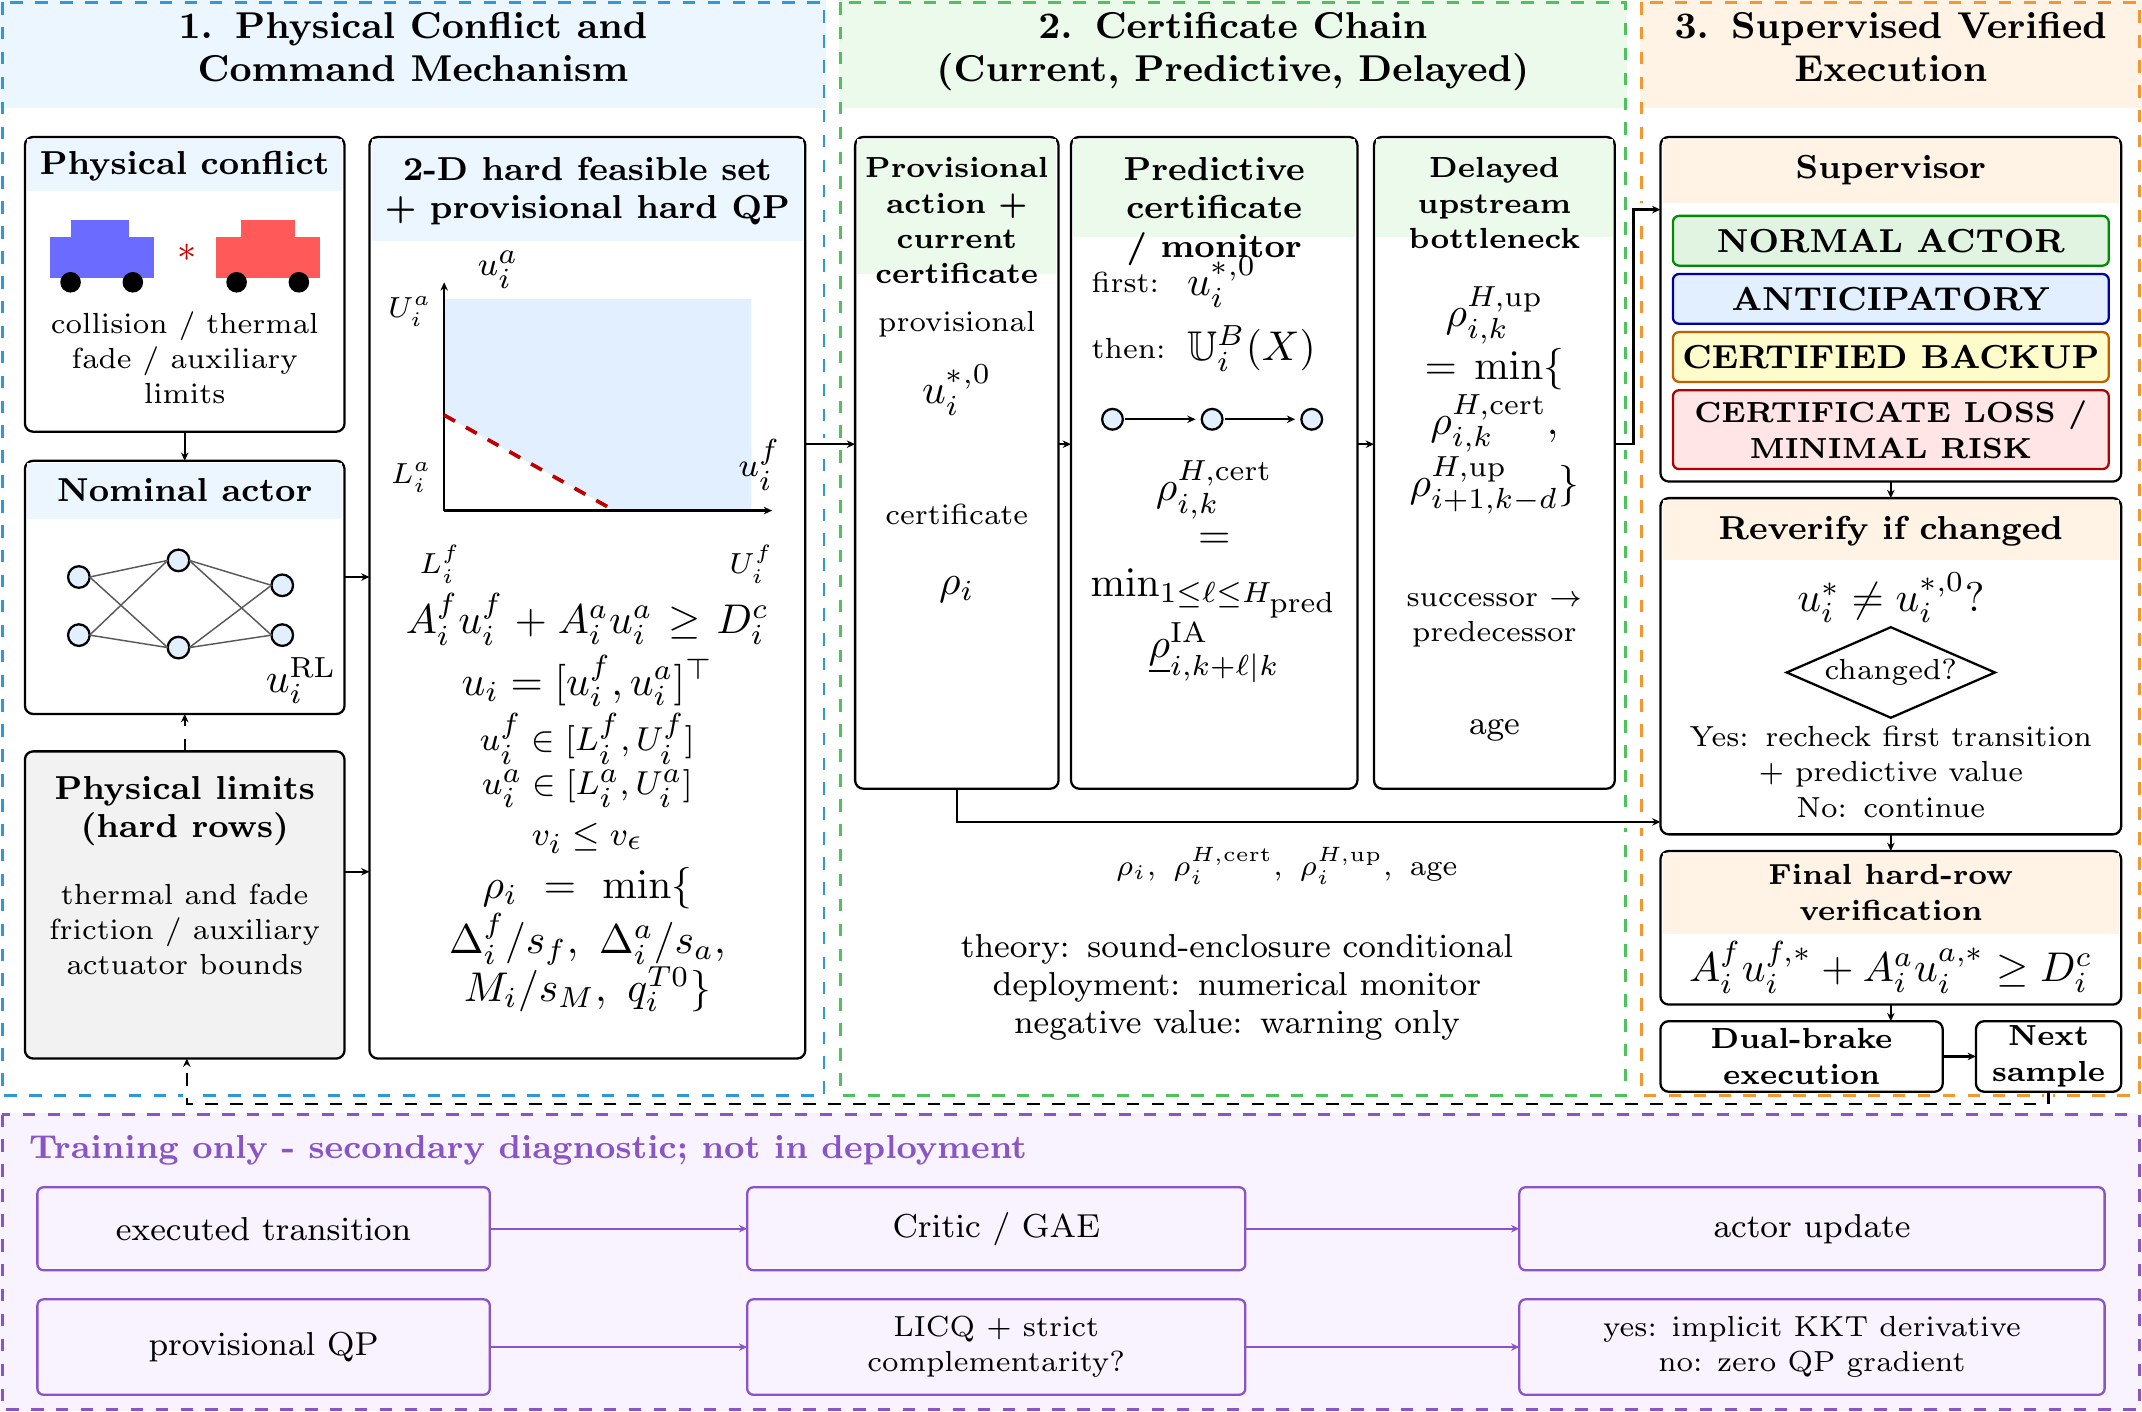
\includegraphics[width=\textwidth]{figures/fig1_desktop66_final.png}
\caption{Certificate-aware dual-brake command mechanism. Collision demand and physical limits define the two-dimensional hard set and instantaneous reserve. The theoretical predictive certificate is conditional on sound enclosure, whereas deployment uses a numerical monitor whose negative value is a warning only. The delayed upstream bottleneck carries age into four-mode supervision. A changed action is reverified before final hard-row verification and execution. The lower strip denotes training-only diagnostics.}
\label{fig:framework}
\end{figure*}

\section{Related Work}
\subsection{Connected Platoons and Brake Physics}
Connected controllers use predecessor/leader information to improve tracking and disturbance attenuation \cite{naus2010string,ploeg2011cacc}. Collision invariance and string stability remain distinct. Brake-temperature studies range from conduction models \cite{talati2009brake} to heavy-platoon fade compensation \cite{devika2022fade}. Li \emph{et al.} optimize composite friction, regenerative, and hydraulic-retarder braking on long descents \cite{li2025retarder}. These works motivate the plant model, but do not certify whether collision demand remains jointly satisfiable with thermally degrading friction and lagged gear/power-limited auxiliary actuation.

\subsection{Safety-Critical Learning and Predictive Certification}
CBF-QPs and high-order control barrier functions (HOCBFs) provide invariance conditions \cite{ames2017cbf,xiao2022hocbf}; differentiable layers are established in safety-critical learning \cite{ma2022differentiable,xiao2023barriernet,yang2023diffcbf}. Connected-vehicle CBF control and event-triggered safe reinforcement learning (RL) address networked and intersample uncertainty \cite{li2025connectedcbf,hu2025event}. Zhou \emph{et al.} combine multi-agent reinforcement learning (MARL), cooperative CBFs, uncertainty prediction, and a differentiable QP for platoons \cite{zhou2026cooperative}; Ohnemus \emph{et al.} study distributed predictive CBF certification and recoverability \cite{ohnemus2026dpcbf}; Sah and Keshavan derive a generic exact CBF feasibility reserve \cite{sah2026exact}; and Guo \emph{et al.} use multi-step reachable-set information in uncertainty-aware CBF-constrained model predictive control (MPC) \cite{guo2025uncertainty}. These works establish the generic safety and optimization tools used here.

The present validation also includes an independent native reimplementation sanity check and an adapted heavy-duty matched comparison with the recent T-ITS method of Zhou \emph{et al.}; this comparison is a domain-transfer stress test rather than a ranking of the methods in their native domains.

The remaining gap is a physics-specific predictive feasibility framework in which collision-braking demand competes with heat/fade-limited friction and lagged gear/power-limited auxiliary braking under sampled commands and communication constraints. Complete interval-plus-coupled-row geometry, finite-horizon interval propagation, and physical bottleneck attribution address that gap. Multi-agent proximal policy optimization (MAPPO) is one centralized-training-and-decentralized-execution (CTDE) nominal-controller substrate \cite{yu2022mappo}; local QP differentiation is a secondary diagnostic. Table~\ref{tab:positioning} compares the scope of closely related work.

\begin{table*}[t]
\caption{Scope relative to closest literature; entries describe explicit focus, not ranking.}
\label{tab:positioning}
\centering\scriptsize
\begin{tabular}{lccccc}
\toprule
Work & Domain & Predictive/reachable & Exact feasibility & Differentiable QP & Coupled thermal dual brake \\
\midrule
Zhou \emph{et al.} \cite{zhou2026cooperative} & mixed platoon & uncertainty prediction & -- & yes & -- \\
Ohnemus \emph{et al.} \cite{ohnemus2026dpcbf} & modular multi-agent & yes & recoverability & -- & -- \\
Sah--Keshavan \cite{sah2026exact} & multi-robot & -- & yes & -- & -- \\
Guo \emph{et al.} \cite{guo2025uncertainty} & autonomous driving & $n$-step set & -- & -- & -- \\
Hu \emph{et al.} \cite{hu2025event} & automated vehicle & intersample & -- & -- & -- \\
Li \emph{et al.} \cite{li2025retarder} & downhill truck & receding horizon & -- & -- & yes \\
This work & heavy platoon & conditional interval tube & complete $\rho$ & local/conditional & yes \\
\bottomrule
\end{tabular}
\end{table*}

\section{Problem Formulation}
Consider a leader indexed by $0$ and $N$ controlled trucks $i\in\{1,\ldots,N\}$ on a road coordinate. Vehicle $i$ has parameter vector
\begin{equation}
\vartheta_i=(m_i,L_i,c_{r,i},C_{d,i}A_i,\tau_i^f,\tau_i^a,C_i,k_i,\eta_i,\bar b_i),
\end{equation}
where $m_i$ is vehicle mass, $L_i$ is vehicle length, $c_{r,i}$ is the rolling-resistance coefficient, $C_{d,i}A_i$ is the aerodynamic drag-area term, $\tau_i^f$ and $\tau_i^a$ are the friction- and auxiliary-brake actuator time constants, $C_i$ is lumped brake thermal capacity, $k_i$ is the cooling coefficient, $\eta_i$ is the specified friction-heating coefficient, and $\bar b_i$ is the cold nominal friction-brake force capability. The physical state and command are
\begin{equation}
x_i=[p_i,v_i,b_i,r_i,T_i]^\top,\qquad
u_i=[u_i^f,u_i^a]^\top,
\end{equation}
where $p_i$ is longitudinal position, $v_i$ is longitudinal speed, $b_i$ and $r_i$ are realized friction- and auxiliary-brake forces, $T_i$ is friction-brake temperature, and $u_i^f$ and $u_i^a$ are the commanded friction- and auxiliary-brake forces. The command vector thus has exactly two QP coordinates, corresponding to friction and auxiliary braking. Tables~\ref{tab:parameters} and~\ref{tab:nomenclature} summarize the per-class parameter provenance and notation used below.
Hard feasibility is not a function of $x_i$ alone because command memory under zero-order hold, gear availability, dwell logic, and communication validity depend on memory. At sample $k$ the controller therefore uses the augmented hybrid state
\begin{equation}\label{eq:chi}
\begin{aligned}
\chi_{i,k}=[&p_{i,k},v_{i,k},b_{i,k},r_{i,k},T_{i,k},
u^f_{i,k-1},u^a_{i,k-1},g_{i,k},\\
&\tau^g_{i,k},a^{\rm msg}_{i,k},d_{i,k},
v_{i-1,k},a_{i-1,k}]^\top .
\end{aligned}
\end{equation}
Here $g_{i,k}$ is the discrete gear state, $\tau^g_{i,k}$ is the elapsed dwell time in that gear state, $a^{\rm msg}_{i,k}$ is the age of the most recently accepted safety message, $d_{i,k}$ is the inter-vehicle bumper gap, and $v_{i-1,k}$ and $a_{i-1,k}$ are predecessor speed and acceleration. The last three quantities are required by the collision row and predecessor reachable tube. Every certificate below is consequently written as a function of $\chi_{i,k}$, not merely $x_i$.

The time-varying directed vehicle-to-vehicle (V2V) communication graph is $\mathcal G_t=(\mathcal V,\mathcal E_t)$. Agent $i$ observes
\begin{equation}
o_i=(v_i,b_i,r_i,T_i,u^f_{i,k-1},u^a_{i,k-1},g_i,\tau_i^g,
\vartheta_i,\hat\theta_i,d_i,\Delta v_i,
\mathcal M_i),
\end{equation}
where $d_i=p_{i-1}-p_i-L_{i-1}$, $\Delta v_i=v_{i-1}-v_i$, $\hat\theta_i$ is the locally estimated road grade, and $\mathcal M_i$ contains time-stamped permitted messages including the age needed for \eqref{eq:chi}. A message generated at $t_g$ and received at $t$ is replaced by a reachable tube $\mathcal R_{i-1}(t-t_g)$ formed from declared acceleration and jerk bounds. Packets inconsistent with local range/range-rate sensing are rejected, and the union of sensing and communication uncertainty is used in the robust margin. The critic uses global state only during training.

The policy must minimize tracking, comfort, braking-energy, coordination, and intervention costs while maintaining collision, temperature, fade, and actuator constraints. Jerk is a soft comfort constraint and therefore never determines the hard safety feasibility claim. Training, identification, validation, and held-out/out-of-distribution (OOD) test sets are disjoint.

At the transport level, a mission contains a descent profile $\theta(p)$, desired speed schedule, fleet order, payloads, ambient condition, and communication trace. We report
\begin{equation}
J_{\rm op}=\left[t_{\rm trip},E_{\rm fric},E_{\rm aux},e_v^{\rm rms},
e_d^{\rm rms},j^{\rm rms},n_{\rm stop}\right],
\end{equation}
where $E_{\rm fric}=\sum_i\int b_iv_i\,dt$ and $E_{\rm aux}=\sum_i\int r_iv_i\,dt$; $e_v^{\rm rms}$, $e_d^{\rm rms}$, and $j^{\rm rms}$ are speed-error, spacing-error, and jerk root-mean-square (RMS) quantities. Safety is reported separately from efficiency so that an unnecessarily slow method cannot appear superior merely because it avoids demanding maneuvers.

String stability is also separate from safety. With spacing error $e_i^d$, the empirical gains are
\begin{equation}
G_{2,i}=\frac{\|e_i^d\|_2}{\|e_{i-1}^d\|_2+\epsilon_g},\qquad
G_{\infty,i}=\frac{\|e_i^d\|_\infty}{\|e_{i-1}^d\|_\infty+\epsilon_g}.
\end{equation}
Here $\epsilon_g>0$ is a small denominator regularizer that prevents division by zero or a near-zero predecessor-error norm; it is not a safety parameter. We test whether $\max_iG_{2,i}\le1$ and $\max_iG_{\infty,i}\le1$ across platoon lengths; no analytical string-stability theorem is claimed.

\begin{table}[t]
\caption{Vehicle Parameters Required Per Class}
\label{tab:parameters}
\centering
\scriptsize
\begin{tabular}{@{}p{0.16\columnwidth}p{0.38\columnwidth}p{0.26\columnwidth}@{}}
\toprule
Group & Parameters & Evidence \\
\midrule
Geometry & $m_i,L_i$, axle/load state & weighed vehicle/configuration \\
Resistance & $c_{r,i},C_{d,i}A_i$ & coast-down or source data \\
Actuator & $\tau_i^f,\tau_i^a,\bar u_i^f,\bar u_i^a(v,g)$ & friction/retarder step and power maps \\
Thermal & $C_i,k_i,\eta_i,T_{\rm crit,i}$ & dynamometer/descent fit \\
Fade & $\phi_i(T)$ and uncertainty & held-out force--temperature curve \\
Derivatives & $\dot\theta,\dot q^w,\dot F^r$, predecessor jerk bounds & held-out extrema or certified limits \\
Safety & $a_i^S,t_{h,i},d_{0,i}$ & validated lower bound/policy \\
\bottomrule
\end{tabular}
\end{table}

\begin{table}[t]
\caption{Core Symbols (SI Units Unless Stated)}
\label{tab:nomenclature}
\centering\scriptsize
\begin{tabular}{@{}lp{0.64\columnwidth}@{}}
\toprule
Symbol & Meaning \\
\midrule
$b,r$ & realized friction and auxiliary brake forces (N) \\
$u^f,u^a$ & commanded friction and auxiliary forces (N) \\
$T,T_a,T_{\rm crit}$ & brake, ambient, and critical temperatures (K) \\
$h^c,h^T,h^F,h^A$ & collision, thermal, fade, and auxiliary barriers \\
$A^f,A^a,D^c$ & collision-row coefficients and demand \\
$[L^f,U^f],[L^a,U^a]$ & effective command intervals after all individual rows \\
$M$ & exact conflict reserve in collision-row units \\
$g^{T0}$ & undivided low-speed state-only thermal reserve (K) \\
$\gamma,\mu$ & directional model and sampled-data margins \\
$H_{\rm QP}$ & safety-QP Hessian; $N_{\rm rec}$ is recovery count \\
\bottomrule
\end{tabular}
\end{table}


Figure~\ref{fig:coupled} summarizes the coupling among friction and auxiliary commands, their actuator lags, longitudinal dynamics, friction heating, and temperature-dependent fade.
\begin{figure*}[t]
\centering
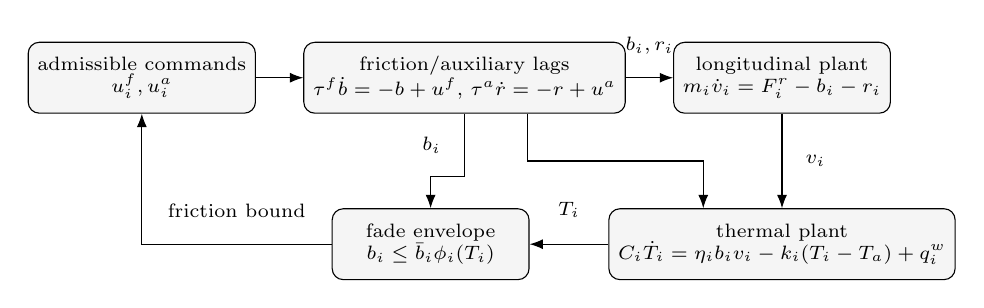
\begin{tikzpicture}[font=\scriptsize,>=Latex,node distance=6mm,
 box/.style={draw,rounded corners,minimum width=25mm,minimum height=9mm,align=center,fill=gray!8}]
\node[box] (cmd) {admissible commands\\$u_i^f,u_i^a$};
\node[box,right=of cmd] (lag) {friction/auxiliary lags\\$\tau^f\dot b=-b+u^f$, $\tau^a\dot r=-r+u^a$};
\node[box,right=of lag] (long) {longitudinal plant\\$m_i\dot v_i=F_i^r-b_i-r_i$};
\node[box,below=12mm of long] (heat) {thermal plant\\$C_i\dot T_i=\eta_i b_i v_i-k_i(T_i-T_a)+q_i^w$};
\node[box,left=10mm of heat] (fade) {fade envelope\\$b_i\le \bar b_i\phi_i(T_i)$};
\draw[->] (cmd)--(lag);
\draw[->] (lag)--node[midway,above=5pt]{$b_i,r_i$}(long);
\draw[->] (lag.south) -- node[midway,left=5pt]{$b_i$} ++(0,-8mm) -| (fade.north);
\draw[->] ([xshift=8mm]lag.south) -- ++(0,-6mm) -| ([xshift=-10mm]heat.north);
\draw[->] (long)--node[midway,right=5pt]{$v_i$}(heat);
\draw[->] (heat)--node[midway,above=6pt]{$T_i$}(fade);
\draw[->] (fade.west) -- node[midway,above=6pt]{friction bound} (cmd.south |- fade.west) -- (cmd.south);
\end{tikzpicture}

\caption{Coupling among friction and auxiliary commands, their distinct actuator lags, longitudinal motion, friction heating, and the temperature-dependent fade envelope.}
\label{fig:coupled}
\end{figure*}

\section{Dynamics and Constraint Geometry}
\subsection{Dual-Brake Longitudinal--Thermal Model}
With positive road angle uphill, define the nonbraking force
\begin{equation}
F_i^r=F_i^d-m_ig\sin\theta_i-m_igc_{r,i}\cos\theta_i-
\tfrac12\rho_{\rm air}C_{d,i}A_iv_i^2+w_i,
\end{equation}
where $\rho_{\rm air}$ is air density, $F_i^d$ is the modeled driveline-force contribution, and $w_i$ is the lumped residual longitudinal force/disturbance term. The model is
\begin{subequations}\label{eq:model}
\begin{align}
\dot p_i&=v_i, & m_i\dot v_i&=F_i^r-b_i-r_i,\\
\tau_i^f\dot b_i&=-b_i+u_i^f,
&\tau_i^a\dot r_i&=-r_i+u_i^a,\\
C_i\dot T_i&=\eta_i b_iv_i-k_i(T_i-T_a)+q_i^w.
\end{align}
\end{subequations}
The auxiliary envelope captures retarder/engine-brake power, shaft-speed, gear, and response restrictions:
\begin{equation}\label{eq:auxenv}
0\le r_i\le\bar r_i(v_i,g_i),\quad
0\le u_i^a\le\bar u_i^a(v_i,g_i).
\end{equation}
Each command is constant on the open zero-order-hold (ZOH) interval and may change at a sample instant. No independent physical command-slew limit is asserted. The realized forces remain continuous through the identified first-order actuator dynamics in \eqref{eq:model}.
Realized-force availability is not implied by the command envelope. Define the longitudinal acceleration $a_i:=\dot v_i$. For a fixed valid gear branch during one ZOH interval, define $h_i^A=\bar r_i(v_i,g_i)-r_i$ and $\bar r_{i,v}:=\partial\bar r_i(v_i,g_i)/\partial v_i$. Its robust CBF gives
\begin{equation}\label{eq:auxcbf}
u_i^a\le r_i+\tau_i^a\!\left[\bar r_{i,v}a_i+\alpha_A(h_i^A)-\gamma_i^A-\mu_i^A\right].
\end{equation}
For permitted shifts, the controller uses the minimum valid envelope over reachable gears and enforces the manufacturer's dwell time; no derivative is taken through a gear discontinuity.
The friction envelope is $0\le b_i\le\bar b_i\phi_i(T_i)$, where $\phi_i'(T)\le0$ on a calibrated interval. Parameters and residual/derivative bounds must be identified on separate data.

The selected functions $\alpha_{1c},\alpha_{2c},\alpha_{1T},\alpha_{2T},\alpha_F$, and $\alpha_A$ are locally Lipschitz extended class-$\mathcal K$ functions on the declared operating domain. Their choices are fixed before evaluation; no gain is inferred from the reported outcomes.

\subsection{Collision HOCBF}
Let $a_i^S>0$ lower-bound follower braking, $a_{i-1}^E>0$ upper-bound predecessor emergency deceleration, and $t_{h,i},d_{0,i}$ denote prescribed time headway and standstill spacing. With $q_i=t_{h,i}+\tau_i^f$,
\begin{equation}\label{eq:hc}
h_i^c=d_i-d_{0,i}-q_iv_i-\frac{v_i^2}{2a_i^S}
+\frac{v_{i-1}^2}{2a_{i-1}^E}.
\end{equation}
Set $c_i=q_i+v_i/a_i^S$ and $r_{i-1}^v=v_{i-1}/a_{i-1}^E$. Then
\begin{align}
\dot h_i^c&=v_{i-1}-v_i-c_ia_i+r_{i-1}^va_{i-1},\label{eq:hcdot}\\
\ddot h_i^c&=a_{i-1}-a_i-\frac{a_i^2}{a_i^S}-c_i\dot a_i
+\frac{a_{i-1}^2}{a_{i-1}^E}+r_{i-1}^v\dot a_{i-1}.\label{eq:hcddot}
\end{align}
The continuous-time jerk is
\begin{equation}\label{eq:jerk}
j_i=\dot a_i=\frac{\dot F_i^r}{m_i}+\frac{b_i-u_i^f}{m_i\tau_i^f}
+\frac{r_i-u_i^a}{m_i\tau_i^a}.
\end{equation}
Hence both commands enter $\ddot h_i^c$ with positive coefficients. For $\psi_{1i}^c=\dot h_i^c+\alpha_{1c}(h_i^c)$, the sampled-data-tightened robust HOCBF is
\begin{equation}\label{eq:collision_hocbf}
A_i^fu_i^f+A_i^au_i^a+\widehat\Xi_i^c-\gamma_i^c-\mu_i^c
+\alpha_{2c}(\psi_{1i}^c)\ge0,
\end{equation}
where $A_i^f=c_i/(m_i\tau_i^f)>0$, $A_i^a=c_i/(m_i\tau_i^a)>0$, and $\mu_i^c$ is the intersample tightening.

\subsection{Temperature HOCBF and Fade CBF}
Let $h_i^T=T_{\rm crit,i}-T_i$. Its first derivative contains no command. Differentiation gives
\begin{equation}
\ddot h_i^T=-\frac{\eta_iv_i}{C_i\tau_i^f}u_i^f+\Xi_i^T,
\end{equation}
where, for constant thermal parameters,
\begin{equation}
\widehat\Xi_i^T=\frac{\eta_ib_iv_i}{C_i\tau_i^f}-\frac{\eta_ib_ia_i}{C_i}
+\frac{k_i}{C_i}(\dot T_i-\dot T_a)-\frac{\widehat{\dot q_i^w}}{C_i}.
\end{equation}
Rather than differentiating noisy heat residuals, implementation bounds $\dot q_i^w$, $\dot T_a$, grade rate, and resistance derivatives. With $\psi_{1i}^T=\dot h_i^T+\alpha_{1T}(h_i^T)$,
\begin{equation}\label{eq:thermal_hocbf}
-B_i^fu_i^f+\widehat\Xi_i^T-\gamma_i^T-\mu_i^T
+\alpha_{2T}(\psi_{1i}^T)\ge0,
\quad B_i^f=\frac{\eta_iv_i}{C_i\tau_i^f}.
\end{equation}
Temperature therefore caps friction braking but does not directly cap auxiliary braking.

The fade envelope is enforced dynamically rather than checked as a state-only row. Define
\begin{equation}
h_i^F=\bar b_i\phi_i(T_i)-b_i.
\end{equation}
The first-order robust CBF $\dot h_i^F+\alpha_F(h_i^F)\ge0$ yields the explicit upper bound
\begin{equation}\label{eq:fade_cbf}
u_i^f\le b_i+\tau_i^f\!\left[\bar b_i\phi_i'(T_i)\dot T_i
+\alpha_F(h_i^F)-\gamma_i^F-\mu_i^F\right].
\end{equation}
Let $v_\epsilon$ denote the specified low-speed switching threshold. At $v_i\le v_\epsilon$, $B_i^f$ is too small for a meaningful division. Under ZOH commands and constant $v_i,T_a,q_i^w$ over $[t_k,t_k+\Delta t]$, set $\lambda_i=k_i/C_i$, $E_i=e^{-\lambda_i\Delta t}$,
\begin{equation}
I_{0i}=\frac{1-E_i}{\lambda_i},\qquad
I_{1i}=E_i\frac{e^{(\lambda_i-1/\tau_i^f)\Delta t}-1}{\lambda_i-1/\tau_i^f},
\end{equation}
using the continuous limits when a denominator vanishes. Exact integration yields
\begin{align}
T_{i,k+1}={}&T_a+E_i(T_{i,k}-T_a)+\frac{q_i^wI_{0i}}{C_i}\nonumber\\
&+\frac{\eta_i v_i}{C_i}\{b_{i,k}I_{1i}+u_{i,k}^f(I_{0i}-I_{1i})\}.\label{eq:zohthermal}
\end{align}
Separate the command-independent prediction
\begin{equation}
T_{i,k+1}^{\rm base}=T_a+E_i(T_{i,k}-T_a)+q_i^wI_{0i}/C_i+\eta_i v_i b_{i,k}I_{1i}/C_i
\end{equation}
and define the undivided state-side thermal reserve
\begin{equation}\label{eq:gT0}
g_{i,k}^{T0}=T_{\rm crit,i}-\Delta_T-\bar e_i^T-T_{i,k+1}^{\rm base}.
\end{equation}
Here $\Delta_T>0$ is the registered temperature safety buffer below $T_{\rm crit,i}$ used by the low-speed one-step thermal constraint.
The low-speed hard row is $c_i^Tu_{i,k}^f\le g_{i,k}^{T0}$, where $c_i^T=\eta_iv_i(I_{0i}-I_{1i})/C_i$. It is retained without division. At $v_i=0$, $c_i^T=0$ exactly and the row becomes the command-independent condition $0\le g_{i,k}^{T0}$; therefore $g_{i,k}^{T0}<0$ is hard infeasibility even if both command intervals and the collision row remain feasible. The term $\bar e_i^T$ is computed by \eqref{eq:zoherror} from registered bounds on $|a|$, $|\dot T_a|$, $|\dot q^w|$, thermal parameters, friction lag, and integration error.

\subsection{Directional Robust and Digital Margins}
Define $\zeta_i$ as the collection of measured local/predecessor states, predecessor acceleration and jerk, message age, packet delay, grade and grade rate, rolling and aerodynamic forces, $q_i^w$ and $\dot q_i^w$, and both actuator lags. The box $\mathcal B_i(\hat\zeta_i)=\prod_j[\hat\zeta_{ij}-\varepsilon_{ij}^-,\hat\zeta_{ij}+\varepsilon_{ij}^+]$ includes sensor error and identified parameter/residual intervals. Packet loss acts through message age and a predecessor reachable tube; if age exceeds its registered horizon, the bound is invalid and the supervisor triggers. If $\widehat\Xi_i^k$ is the computed uncontrolled term and $\Xi_i^k$ is the true term, the correct one-sided margin is
\begin{equation}\label{eq:margin}
\gamma_i^k\ge\sup_{\zeta\in\mathcal B_i(\hat\zeta_i)}
\{\widehat\Xi_i^k-\Xi_i^k(\zeta)\},\quad k\in\{c,T,F,A\}.
\end{equation}
Thus $\widehat\Xi_i^k-\gamma_i^k\le\Xi_i^k$; an absolute-error bound is sufficient but unnecessarily conservative. In the theoretical construction, a sound interval arithmetic (IA) lower endpoint $\underline\Xi_i^k$ gives $\gamma_i^k=\max\{0,\widehat\Xi_i^k-\underline\Xi_i^k\}$. The present floating-point implementation has no verified directed-rounding enclosure. Measurement intervals cover position, speed, acceleration, and brake-state sensing; dynamics intervals cover grade/grade rate, resistance, aerodynamics, heat residual/rate, and lag uncertainty; communication intervals cover age/delay plus reachable acceleration/jerk. Each digital rate bound $L_i^k$ is computed by the executable product-rule expression \eqref{eq:ratebound}, and $\mu_i^k=L_i^k\Delta t+\bar e_{\rm int,i}^k$. Empirical quantiles are not used as deterministic bounds.

\section{Certificate-Aware Dual-Brake Control}
\subsection{Hard Safety Polytope and Viability Reserve}
The canonical forward decision is exactly $u_i=[u_i^f,u_i^a]^\top\in\mathbb R^2$. Jerk is evaluated as a comfort metric after the action is applied; it is neither a QP coordinate nor a slack variable. The hard projection is
\begin{subequations}\label{eq:qp}
\begin{align}
u_i^*=\arg\min_{u_i\in\mathbb R^2}\;&\tfrac12(u_i-u_i^{\rm RL})^\top W_i(u_i-u_i^{\rm RL})
+\epsilon\|u_i\|^2\\
\mathrm{s.t.}\;&\eqref{eq:collision_hocbf},\ \eqref{eq:thermal_hocbf},\ \eqref{eq:fade_cbf},\ \eqref{eq:auxcbf},\\
&0\le u_i^f\le\bar u_i^f,\quad 0\le u_i^a\le\bar u_i^a(v_i,g_i),\\
&c_i^Tu_i^f\le g_{i,k}^{T0}\ \text{when }v_i\le v_\epsilon.
\end{align}
\end{subequations}
Here $u_i^{\rm RL}$ is the nominal preprojection command supplied by the policy used in this implementation; the certificate and hard QP accept any nominal command in the declared bounds. $W_i\succeq0$ is the command weighting and $\epsilon>0$ the regularizer, so $H_{{\rm QP},i}=W_i+2\epsilon I\succ0$. No hard row has slack in certified operation.

For $v_i>v_\epsilon$, the thermal HOCBF contributes to the friction interval; for $v_i\le v_\epsilon$, it is replaced, not supplemented, by the undivided ZOH row. All command-dependent noncollision rows reduce to individual intervals $u_i^f\in[L_i^f,U_i^f]$ and $u_i^a\in[L_i^a,U_i^a]$: the friction interval intersects command magnitude, active thermal-mode, and fade bounds; the auxiliary interval intersects command magnitude, gear/power, and realized-force-CBF bounds. For $0<v_i\le v_\epsilon$, $c_i^T>0$ and the ZOH row is absorbed by $U_i^f=\min\{U_i^{f,\mathrm{other}},g_{i,k}^{T0}/c_i^T\}$; at $v_i=0$ it is the state-only gate $g_{i,k}^{T0}\ge0$. The collision row is the sole command-coupled face,
\begin{equation}\label{eq:collisiondemand}
A_i^fu_i^f+A_i^au_i^a\ge D_i^c,\quad
D_i^c=\gamma_i^c+\mu_i^c-\widehat\Xi_i^c-\alpha_{2c}(\psi_{1i}^c).
\end{equation}
The physical collision-demand reserve is
\begin{equation}\label{eq:reserve}
M_i(\chi_{i,k})=A_i^fU_i^f+A_i^aU_i^a-D_i^c.
\end{equation}
It remains interpretable if an individual interval is empty, but its sign alone is then insufficient. Define $\Delta_i^f=U_i^f-L_i^f$, $\Delta_i^a=U_i^a-L_i^a$, and
\begin{equation}
q_{i,k}^{T0}=\begin{cases}g_{i,k}^{T0}/s_{T0},&v_i\le v_\epsilon,\\+\infty,&v_i>v_\epsilon,\end{cases}
\end{equation}
where $s_{T0}>0$ is a fixed temperature scale. With fixed positive normalizers $s_f$ [N], $s_a$ [N], and $s_M$ [m/s$^2$], define the complete signed certificate
\begin{equation}\label{eq:rho}
\rho_i(\chi_{i,k})=\min\!\left\{\Delta_i^f/s_f,\Delta_i^a/s_a,M_i(\chi_{i,k})/s_M,q_{i,k}^{T0}\right\}.
\end{equation}
We fix $s_f$ to reference cold friction-force capability, $s_a$ to reference auxiliary-force capability, $s_M$ to a reference deceleration/barrier-row scale, and $s_{T0}$ to a fixed one-step temperature scale. They are shared by every algorithm and never retuned per method. Positive choices preserve the sign but affect magnitude, trigger time, learning loss, and the normalized critical component; therefore $\Delta_i^f$, $\Delta_i^a$, $M_i$, and low-speed $g_{i,k}^{T0}$ are always logged and evaluated in a fixed scale-sensitivity study. Instantaneous feasibility is
\begin{equation}\label{eq:instantfeas}
\mathsf{Feas}_{i,k}:=(\rho_i(\chi_{i,k})\ge0).
\end{equation}
Thus nonnegative $M_i$ never hides an empty interval or a failed zero-coefficient thermal row: $M_i$ remains the physical collision supply-minus-demand term, while $\rho_i$ is the complete exact certificate. For fixed auxiliary command,
\begin{align}
u_i^f&\ge\ell_i^c(u_i^a)=\frac{D_i^c-A_i^au_i^a}{A_i^f},\label{eq:lower}\\
u_i^f&\le U_i^f.\label{eq:upper}
\end{align}
The exact minimum in \eqref{eq:rho} is used for certification; only the learning path may smooth it.

\subsection{Predictive Feasibility Formulation and Distributed Bottleneck Monitoring}
Let $H_{\rm pred}$ be the theoretical predictive horizon in samples and $\mathcal X^B_{i,k\mid k}=\{\chi_{i,k}\}$. At step $\ell$, let $\Omega_\ell$ be the declared uncertainty box and $\mathbb U_i^B(\mathcal X)$ a sound set-valued command enclosure of the pointwise backup law $\kappa_i^B$, so $\{\kappa_i^B(\chi):\chi\in\mathcal X\}\subseteq\mathbb U_i^B(\mathcal X)$. Under the sound-enclosure assumption, the closed-loop tube obeys
\begin{equation}\label{eq:tube}
\mathcal X^B_{\ell+1}\supseteq\mathcal F_i^{\rm IA}(\mathcal X^B_\ell,\mathbb U_i^B(\mathcal X^B_\ell),\Omega_\ell).
\end{equation}
Table~\ref{tab:predictive_symbols} summarizes the predictive and learning notation, including the learning horizon $H_L$ in samples. Table~\ref{tab:constraints} distinguishes the hard projection rows from quantities, such as jerk, that lie outside the hard QP.
In the theoretical construction, $\mathcal F_i^{\rm IA}$ must be a sound outward interval extension of the sampled plant, including all admissible discrete branches; $\Omega_\ell$ covers the declared plant, predecessor, thermal, gear, and communication uncertainty. The first transition uses the provisional hard-QP solution $u_{i,k}^{*,0}$. For $\ell\ge2$, $\mathbb U_i^B(\mathcal X)$ must enclose all pointwise backup commands, componentwise as an outward-rounded interval enclosure. A midpoint or center-point backup trajectory is not certified. The evaluated implementation uses native floating-point interval endpoints and an affine-saturation backup with fixed gear; directed rounding, complete gear/dwell branch hulls, and a global enclosure proof for its reserve callback are not established. Its numerical predictive output is therefore an empirical warning diagnostic, not a formally assured enclosure. Backup-command interval widths are logged.

For comparison define the generally intractable true robust reserve
\begin{equation}
\rho_{i,k}^{H,{\rm true}}=\min_{1\le\ell\le H_{\rm pred}}\inf_{\chi\in\mathcal X^B_{i,k+\ell\mid k}}\rho_i(\chi).
\end{equation}
Under sound enclosure, the interval evaluation supplies a lower bound,
\begin{align}
\underline\rho^{\rm IA}_{i,k+\ell\mid k}
&\le\inf_{\chi\in\mathcal X^B_{i,k+\ell\mid k}}\rho_i(\chi),\label{eq:predlower}\\
\rho_{i,k}^{H,{\rm cert}}
&=\min_{1\le\ell\le H_{\rm pred}}\underline\rho^{\rm IA}_{i,k+\ell\mid k}.\label{eq:rhocert}
\end{align}
Under the stated sound-enclosure assumption, $\rho^{H,{\rm cert}}\ge0$ certifies robust hard feasibility. A negative value is an inconclusive conservative warning unless exact reachable-set optimization proves equality. The current numerical monitor has not been shown to satisfy that assumption; it records the minimizing step and physical row for diagnostic use.

For the theoretical certificate, the centralized minimum is
\begin{equation}\label{eq:fleetreserve}
\rho_{{\rm fleet},k}^{H,{\rm cert}}=\min_i\rho_{i,k}^{H,{\rm cert}},
\end{equation}
and is used only by centralized training/evaluation. Deployment uses successor-to-predecessor recursive aggregation
\begin{align}
\rho_{i,k}^{H,{\rm up}}&=\min\{\rho_{i,k}^{H,{\rm cert}},\rho_{i+1,k-d}^{H,{\rm up}}\},\label{eq:minconsensus}\\
m_{i,k}^{\rm safe}&=(\rho_{i,k}^{H,{\rm up}},i_{\rm crit},\ell_{\rm crit},q_{\rm crit},t_k),
\end{align}
Here $d$ is the accepted message delay/age in samples, while $i_{\rm crit}$, $\ell_{\rm crit}$, and $q_{\rm crit}$ identify the critical vehicle, prediction step, and physical certificate row attaining the recursive minimum. A missing or over-age message is replaced by the declared conservative communication-age bound, not ignored. Consequently a truck knows only its age-bounded local/upstream aggregate; it does not instantly know the exact global minimum.

\begin{table}[t]
\caption{Predictive and learning symbols.}
\label{tab:predictive_symbols}
\centering\scriptsize
\begin{tabular}{ll}
\toprule
Symbol & Definition \\
\midrule
$H_{\rm pred}$ & theoretical predictive horizon (samples) \\
$H_L$ & differentiable learning horizon (samples) \\
$\tau_s>0$ & learning soft-min temperature \\
$\mathcal F^{\rm IA}$ & theoretical sound interval set map \\
$\Omega_\ell$ & declared uncertainty box at step $\ell$ \\
$\kappa^B,\mathbb U^B$ & point backup and command-set extension \\
$\epsilon_{\rm th},\epsilon_\tau$ & thermal-parameter and lag relative bounds \\
$s_f,s_a,s_M,s_{T0}$ & fixed physical certificate normalizers \\
$\rho_{\rm pred,trig},\rho_{\rm hard,trig}$ & predictive and hard trigger levels \\
$\rho_{\rm pred,rec},\rho_{\rm hard,rec}$ & hysteretic recovery levels \\
$N_{\rm rec}$ & consecutive recovery samples \\
\bottomrule
\end{tabular}
\end{table}


\begin{table}[t]
\caption{Projection Constraints and Guarantee Status}
\label{tab:constraints}
\centering
\scriptsize
\begin{tabular}{@{}p{0.23\columnwidth}p{0.15\columnwidth}p{0.42\columnwidth}@{}}
\toprule
Constraint & Default & Consequence of relaxation \\
\midrule
Spacing HOCBF & hard & positive slack removes strict collision claim \\
Thermal HOCBF & hard & positive slack removes thermal invariance claim \\
Fade CBF & hard & positive slack removes fade-envelope invariance \\
Friction/auxiliary envelopes & hard & relaxation can request unavailable force/power \\
Auxiliary envelope and realized-force CBF & hard & relaxation can violate lag/gear availability \\
Low-speed ZOH thermal row & hard & relaxation removes the near-stop thermal claim \\
Jerk & outside QP & comfort metric; not part of hard feasibility \\
Tracking objective & soft & performance degradation only \\
\bottomrule
\end{tabular}
\end{table}


\subsection{Secondary Learning Diagnostic}
Under CTDE, a parameter-shared actor samples $\epsilon_i\sim\mathcal N(0,I)$ and $y_i=\mu_\theta(o_i)+\sigma_\theta(o_i)\odot\epsilon_i$, then maps each component to physical nominal bounds by $u_{ij}^{\rm RL}=l_{ij}+(h_{ij}-l_{ij})(\tanh y_{ij}+1)/2$. The stored nominal log density includes the Gaussian term and the $\tanh$/affine Jacobian. Proximal policy optimization (PPO) ratios therefore refer to the nominal sample, while the centralized critic and generalized advantage estimation (GAE) use the executed command $u_i^*$ and its resulting transition.

The paired diagnostic augments the usual clipped PPO objective with an intervention term
\begin{equation}\label{eq:actorloss}
\mathcal J_\theta=\mathcal L_{\rm clip}+\beta\mathcal H(\pi_\theta)
-\lambda_I\mathbb E\|u_i^{*,0}-u_i^{\rm RL}\|_{W_i}^{2}.
\end{equation}
Here $\beta\ge0$ is the entropy-regularization weight and $\lambda_I\ge0$ is the weight of the fixed intervention penalty.
Both matched branches use the same nominal sample, reward, two-dimensional forward QP, executed transition, critic target, and optimizer schedule. DiffQP differentiates the provisional output $u_i^{*,0}$ in the intervention term only when the regularity gates below pass; StopGradient detaches only that output path. The direct dependence on $u_i^{\rm RL}$ is retained in both. Certified interval extrema, supervisor decisions, messages, backup switches, and physical dynamics are stop-gradient quantities. Reward terms never replace hard rows.

\subsection{Karush--Kuhn--Tucker (KKT) Differentiation}
Write the strongly convex two-variable safety QP as $\min_u u^\top H_{\rm QP}u/2-(Bp+h)^\top u$ subject to $Gu\le q$, where $G$ stacks the inequality-constraint rows and $q$ is their bound vector. For the forward projection, $p:=u^{\rm RL}$, $H_{\rm QP}:=W+2\epsilon I$, $B:=W$, and $h:=0$; the omitted term $p^\top Wp/2$ is constant in $u$. Let $\mathcal A$ index the active inequality rows. For an active set satisfying the linear independence constraint qualification (LICQ) and strict complementarity,
\begin{equation}\label{eq:kktdiff}
\begin{bmatrix}H_{\rm QP}&G_{\mathcal A}^\top\\G_{\mathcal A}&0\end{bmatrix}
\begin{bmatrix}\partial u^*/\partial p\\\partial\lambda_{\mathcal A}^*/\partial p\end{bmatrix}
=\begin{bmatrix}B\\0\end{bmatrix}.
\end{equation}
At active-set switches or nonregular active sets, a classical derivative need not exist. LICQ requires the active row gradients to be linearly independent. Because $u\in\mathbb R^2$, more than two simultaneously active inequality gradients cannot all be linearly independent. The calibrated learning scenarios commonly activate four rows and are therefore structurally degenerate for this local active-set KKT representation. The forward QP remains valid and solved; only the selected local derivative is unavailable. A predefined zero-gradient fallback returns zero QP-mediated gradient while preserving the forward action. Separate regular-case tests verify the local derivative against finite differences; the formal learning outcome is summarized in the Results section.

\subsection{Supervisory Backup and Recovery}
Define the backup-feasible domain
\begin{equation}
\begin{split}
\mathcal K_i^B=\{\chi_i:\;&h_i^c,h_i^T,h_i^F,h_i^A,\psi_{1i}^c,\psi_{1i}^T,\rho_i,v_i\ge0,\\
&q_i^{\rm gear/dwell}=1,\ q_i^{\rm comm}=1\},
\end{split}\label{eq:backupdomain}
\end{equation}
where the two Boolean mode indicators mean that gear/dwell logic is admissible and the declared communication uncertainty bound remains valid. The auxiliary state barrier $h_i^A\ge0$ is not implied by the command interval and is therefore explicit. Choose fixed dimensionless thresholds $\rho_{\rm pred,trig}>\rho_{\rm hard,trig}\ge0$ and recovery levels $\rho_{\rm pred,rec}>\rho_{\rm pred,trig}$ and $\rho_{\rm hard,rec}>\rho_{\rm hard,trig}$. The supervisor has four modes: (i) NORMAL ACTOR; (ii) ANTICIPATORY when the evaluated predictive monitor is at or below $\rho_{\rm pred,trig}$, applying early auxiliary braking, headway expansion, and an upstream request; (iii) CERTIFIED BACKUP when $\rho_i\le\rho_{\rm hard,trig}$ or a hard residual fails; and (iv) CERTIFICATE LOSS/MINIMAL RISK when $\rho_i<0$. Recovery requires $N_{\rm rec}$ consecutive samples above both recovery levels.

If the backup hard polytope is empty, no controller using the declared actuators can guarantee all constraints. The minimal-risk mode commands maximum feasible auxiliary braking, caps friction at the temperature/fade bound, requests upstream deceleration and headway expansion, and initiates a controlled stop; it records loss of certificate rather than silently using safety slack.

\subsection{Training and Execution Algorithm}
The executable two-pass order is: (1) measure/time-align state and messages; (2) construct robust/digital margins and hard command intervals; (3) obtain a nominal command $u_{i,k}^{\rm RL}$; (4) solve the normal hard QP for provisional $u_{i,k}^{*,0}$; (5) compute instantaneous $\rho_i$ and propagate the numerical predictive tube using $u_{i,k}^{*,0}$ first and $\mathbb U_i^B(\mathcal X)$ thereafter; (6) evaluate the numerical counterpart of $\rho_i^{H,{\rm cert}}$, physical attribution, the age-bounded recursive bottleneck, and supervisor mode; (7) keep $u^{*,0}$ in NORMAL, otherwise solve the anticipatory QP or backup; (8) if final $u_i^*\ne u_i^{*,0}$, re-evaluate the first transition and predictive value or run the equivalent fast verifier; (9) validate every final hard-row residual and apply $u_i^*$; and (10) log nominal, provisional, final, and both provisional/final predictive values. The implementation exposes this order as one non-reorderable routine. Deployment removes the critic and privileged centralized minimum.

\section{Safety and Predictive-Feasibility Analysis}
\textbf{Assumption 1 (regular bounded model):} On a compact operating domain, \eqref{eq:model} is locally Lipschitz; masses, lags, and heat capacities are bounded away from zero; directional and digital margins dominate all declared estimation, derivative, communication, integration, and sampled-model errors.

\textbf{Assumption 2 (valid backup tube):} $\Omega_{k:k+H}$ contains the true grade/grade rate, predecessor acceleration/jerk, mass/resistance, actuator lags, thermal/fade error, ambient variation, heat-flow residual, gear/power availability, and message age/delay. The first set transition uses the already computed provisional $u_{i,k}^{*,0}$; later transitions use a sound command-set extension $\mathbb U_i^B(\mathcal X)$ of the state-feedback backup. If the supervisor changes the applied command, the first transition is re-evaluated before application.

\textbf{Proposition 1 (complete instantaneous equivalence):} Under the two individual intervals, the coupled row in \eqref{eq:collisiondemand}, and the active low-speed state gate \eqref{eq:gT0}, the hard command set is nonempty if and only if $\rho_i(\chi_{i,k})\ge0$.

\emph{Proof:} All normalizers are positive. At $v_i>v_\epsilon$, $q_{i,k}^{T0}=+\infty$ and the three command-dependent terms give the result. For $0<v_i\le v_\epsilon$, exact zero-order-hold integration gives $c_i^T=\eta_i v_i(I_{0i}-I_{1i})/C_i>0$. Write $U_i^{f,\mathrm{other}}$ for the upper friction bound before the low-speed thermal row and set
\begin{equation}\label{eq:low-speed-upper}
U_i^{f,\mathrm{LS}}=\min\{U_i^{f,\mathrm{other}},g_{i,k}^{T0}/c_i^T\}.
\end{equation}
The $U_i^f$ used in $\Delta_i^f$ and $M_i$ is this intersection in the low-speed branch. Hence the undivided row is satisfied by every $u_i^f\le U_i^f$; $g_{i,k}^{T0}\ge0$ also remains the explicit state-side gate in the implemented certificate. At $v_i=0$, $c_i^T=0$, division is not performed, and the row is exactly the state-only condition $0\le g_{i,k}^{T0}$. At every speed, the command intervals are nonempty precisely when $\Delta_i^f,\Delta_i^a\ge0$. Since $A_i^f,A_i^a>0$, the collision left side is maximal at $(U_i^f,U_i^a)$ and meets demand precisely when $M_i\ge0$. These conditions are exactly the nonnegative components of $\rho_i$; reversing each step proves necessity.

\textbf{Proposition 2 (one-sided robust certificate):} Under Assumption 2, if $\rho_{i,k}^{H,{\rm cert}}\ge0$, then the hard command set is nonempty at every predicted sample for every declared realization.

\emph{Proof:} Sound set propagation places every closed-loop realization in $\mathcal X^B_{i,k+\ell\mid k}$. By \eqref{eq:predlower}, $\rho_i(\chi_{i,k+\ell})\ge\inf_{\chi\in\mathcal X^B}\rho_i(\chi)\ge\underline\rho^{\rm IA}_{i,k+\ell\mid k}\ge\rho_{i,k}^{H,{\rm cert}}$. Proposition 1 applies. Conversely, $\rho_{i,k}^{H,{\rm cert}}<0$ is inconclusive because dependency inflation can lower the interval evaluation below the true infimum. This establishes neither global nor post-horizon recursive feasibility.

\textbf{Proposition 3 (horizon monotonicity):} For a common stored prefix of IA lower bounds, $\rho_i^{H+1,{\rm cert}}\le\rho_i^{H,{\rm cert}}$.

\emph{Proof:} The longer-horizon minimum contains every old lower bound and one additional term.

\textbf{Proposition 4 (closed-loop uncertainty monotonicity):} Let $\Omega_1\subseteq\Omega_2$. Suppose $\mathcal F^{\rm IA}$ is inclusion monotone in state, command, and uncertainty sets, and $\mathbb U^B$ is an inclusion-monotone set extension of the state-feedback backup. Starting from the same singleton, the resulting tubes are nested and $\rho_i^{H,{\rm cert}}(\Omega_2)\le\rho_i^{H,{\rm cert}}(\Omega_1)$ whenever the IA certificate evaluator is inclusion antitone under set enlargement.

\emph{Proof:} Induction: equal initial sets are nested. If $\mathcal X_{1,\ell}\subseteq\mathcal X_{2,\ell}$, inclusion monotonicity gives $\mathbb U^B(\mathcal X_{1,\ell})\subseteq\mathbb U^B(\mathcal X_{2,\ell})$ and then $\mathcal X_{1,\ell+1}\subseteq\mathcal X_{2,\ell+1}$. Lower interval endpoints cannot increase under the stated antitone evaluator; the horizon minimum preserves order. The executable affine-plus-saturation backup satisfies these properties and is regression-tested. No theorem is asserted for an arbitrary non-monotone custom enclosure.

\textbf{Proposition 5 (centralized and recursive minima):} The centralized $\rho_{{\rm fleet},k}^{H,{\rm cert}}\ge0$ if and only if every truck certificate is nonnegative. With zero-delay complete chain delivery, recursive \eqref{eq:minconsensus} at the head equals that centralized minimum and propagates an attaining argmin. With delay/loss it is instead an age-bounded local/upstream quantity using the registered conservative stale-message replacement.

\emph{Proof:} The centralized statement follows from the finite minimum. Recursive pairwise minima are associative and propagate the chosen metadata. Stale replacement changes the operand, so equality with the instantaneous centralized minimum is not claimed.

\textbf{Corollary (physical sensitivities):} Holding all other limits fixed, increasing $U_i^a$ cannot decrease $M_i$, and increasing either individual upper bound cannot decrease $\rho_i$. If the calibrated fade map and every temperature-dependent friction upper bound are nonincreasing in $T_i$, increasing initial temperature cannot increase $\rho_i$. Nested grade or age uncertainty cannot increase $\rho_i^{H,{\rm cert}}$ only under Proposition 4's inclusion assumptions. No monotonicity is asserted when other state-dependent terms change simultaneously.

\textbf{Proposition 6 (sampled-data preservation):} Let each held-command barrier left-hand side $F_i^q$, $q\in\{c,T,F,A\}$, obey $|\dot F_i^q|\le L_i^q$ and have integration error $\bar e_i^q$. Tightening by $\mu_i^q=L_i^q\Delta t+\bar e_i^q$ preserves the continuous row between samples. The executable product-rule bound is
\begin{equation}\label{eq:ratebound}
L_i^q=\bar\xi_{q,\dot{}}+\sum_j(\bar a_{qj}\bar{\dot u}_j+\bar{\dot a}_{qj}\bar u_j),
\end{equation}
with separately registered component bounds for collision, thermal, fade, and auxiliary rows. During each open ZOH interval, $\dot u_j=0$, so the implemented held-command specialization is $L_i^q=\bar\xi_{q,\dot{}}+\sum_j\bar{\dot a}_{qj}\bar u_j$; command jumps are evaluated anew at sample instants.

\emph{Proof:} If the computed sample-time row satisfies the tightened margin $\mu_i^q=L_i^q\Delta t+\bar e_i^q$, the declared error bound gives the true row $F_i^q(t_k)\ge L_i^q\Delta t$. Hence, for every $t\in[t_k,t_k+\Delta t]$, the rate bound gives $F_i^q(t)\ge F_i^q(t_k)-L_i^q(t-t_k)\ge0$. This conclusion is conditional on the declared rate/error bounds and calibrated uncertainty domain; command jumps are checked again at sample instants. The low-speed ZOH thermal branch is handled separately by its registered one-step bound below.

At low speed, variation of the frozen-$v,T_a,q^w$ ZOH prediction is bounded in code and paper by
\begin{align}
\bar e_T={}&\frac{\Delta t^2}{2C_{\min}}\!\left[\eta(\bar b\bar a+\bar v\bar{\dot b})+k\bar{\dot T}_a+\bar{\dot q}^w\right]\nonumber\\
&+\frac{\Delta t\epsilon_{\rm th}}{C_{\min}}\left(\eta\bar b\bar v+k\bar{\dot T}_a\Delta t+\bar{\dot q}^w\Delta t\right)\nonumber\\
&+\frac{\Delta t^2\eta\bar v(\bar u^f+\bar b)\epsilon_\tau}{2C_{\min}\tau_{f,\min}}+\bar e_{\rm int},\label{eq:zoherror}
\end{align}
In the sampled-data and low-speed error bounds, an overbar on a rate or magnitude denotes its registered nonnegative upper or absolute bound over the declared operating domain; physical upper-envelope functions retain their established meanings. Here $C_{\min}>0$ is the registered lower bound on thermal capacity over the declared uncertainty set, $\bar e_{\rm int}$ is the registered numerical-integration and sampled-model error bound, $\bar{\dot b}=(\bar u^f+\bar b)/\tau_{f,\min}$, and $\tau_{f,\min}=\tau_f(1-\epsilon_\tau)$. The ZOH row uses this computed $\bar e_T$, not an unspecified constant.

\textbf{Proposition 7 (QP uniqueness and local sensitivity):} If $H_{\rm QP}\succ0$ and the hard set is nonempty, the two-dimensional primal solution is unique. If the selected active rows additionally satisfy LICQ and strict complementarity, the solution is locally differentiable and \eqref{eq:kktdiff} gives its derivative. Because active gradients lie in $\mathbb R^2$, any active set containing more than two inequality rows is necessarily linearly dependent. At a switch or nonregular set the implementation preserves the forward solution and applies the predefined zero-QP-gradient fallback; it does not assert a classical derivative. No gradient is taken through interval extrema or discrete supervisor modes.

\subsection{Limits of the Claims}
The analysis does not prove that the backup domain is nonempty for every grade, load, initial temperature, emergency maneuver, or horizon extension. It does not prove string stability, global recursive feasibility, empirical superiority, or safety outside calibrated uncertainty. No time-to-conflict theorem is included because no certified global Dini/Clarke derivative bound is available.

\section{Validation Protocols}
\subsection{Literature-Calibrated Physical Model}
The vehicle is a traceable cross-source heavy-duty composite, not an experimentally identified individual truck. Mass, braking force, thermal capacity, and cooling follow the National Highway Traffic Safety Administration (NHTSA) heavy-truck S-cam report \cite{nhtsa2010scam}; total length follows the American Association of State Highway and Transportation Officials (AASHTO) design vehicle \cite{aashto2004}; resistance and drag use a Class-8 study \cite{wang2015fuel}; acceleration and friction-lag bounds use heavy-truck records \cite{vegamoor2018,yanakiev1998}; the auxiliary lag and digitized retarder map use published heavy-truck models \cite{li2026retarder,donkers2020powertrain}; the representative fade curve is digitized from a National Transportation Safety Board (NTSB) study \cite{ntsb2002simulation}; ambient and the independent thermal-discrepancy model use \cite{yan2018thermal}; and communication ranges use field measurements \cite{hu2021delay,gao2016dsrc}. The 10\% and 1-km descent benchmark follows \cite{devika2022fade}. Table~\ref{tab:final-parameters} is generated from the provenance registry.

\begin{table*}[!t]
\centering\scriptsize
\caption{Selected literature-calibrated parameters; full intervals and source-level provenance are archived with the configuration.}
\label{tab:final-parameters}
\begin{tabular}{lllll}
\toprule
Parameter & Symbol & Nominal & SI unit & Provenance \\
\midrule
Vehicle mass & $m$ & 33200 & kg & DIRECT \\
Maximum friction force & $\bar u^f$ & 123603 & N & DERIVED \\
Friction actuator lag & $\tau_f$ & 0.14 & s & DIRECT \\
Auxiliary actuator lag & $\tau_a$ & 0.25 & s & DERIVED \\
Lumped thermal capacity & $C$ & 15439.7 & J/K & DERIVED \\
Cooling coefficient & $k$ & 624.334 & W/K & DERIVED \\
Critical brake temperature & $T_{\rm crit}$ & 463.708 & K & DERIVED \\
Ambient temperature & $T_a$ & 298.15 & K & DIRECT \\
Nominal residual heat & $q_w$ & 0 & W & DERIVED \\
\bottomrule
\end{tabular}
\end{table*}


The validation campaign contains ten studies specified before evaluation: M1 physical feasibility, M2 long-descent allocation, M3 hot-brake conflict, M4 predictive warning, M5 horizon dependence, M6 endpoint and joint design sensitivity, M7 delayed communication, M8 low-speed branch behavior, M9 numerical string stability, and M10 computation time. All 92 campaign runs passed integrity checks. The 20 joint M6 samples are a seeded design-sensitivity set, not draws from a physical probability distribution. A separate follow-up contains 81 boundary-approach scenarios plus the M7 diagnosis; no physical parameter or supervisor threshold was retuned.

For the boundary study, we evaluate the same instantaneous hard rows on a $25\times51$ grid of initial temperature (365--461~K, 4-K increments) and bumper gap (15--90~m, 1.5-m increments) at 15~m/s and a 10\% downgrade. Friction-only feasibility fixes $u_i^a=0$ in the same two-command geometry; dual-brake feasibility retains its physical auxiliary interval. This is an initial command-domain comparison, not a closed-loop campaign. A same-plant supervisor ablation evaluates three 10-s, three-truck scenarios with identical nominal allocator, physical limits, initial states, leader trace, channel, and sampling; the comparator disables only predictive/upstream triggering while retaining instantaneous hard-QP projection. Fixed 50-, 100-, 200-, and 300-ms channel cases use the M7 plant and policy to evaluate head-truck reserve deviation and critical attribution against an instantaneous centralized oracle. The 300-point stratified design varies only nondegenerate declared parameter intervals and the fade digitization offset around one boundary state; it is a deterministic sensitivity design, not a probability law. Source CSV rows and generating scripts accompany these analyses.

The predictive evidence is organized by: (P1) instantaneous versus horizon certificate, (P2) vehicle--time certificate map, (P3) centralized versus recursively available fleet bottleneck, and (P4) physical-limit attribution. Only evaluated, provenance-checked results are reported; planned but unexecuted plots are not treated as evidence.

\subsection{Secondary Matched Learning Protocol}
The ten-seed DiffQP/StopGradient diagnostic matches initialization, random streams, scenario order, reward, optimization budget, forward QP, executed action, and evaluation seeds. Each run uses 20 updates, 12 steps per update, two policy-optimization epochs, and three trucks. Its only intended difference is whether the provisional QP output contributes a valid implicit derivative to the intervention objective; nonregular samples use a zero-QP-gradient fallback. The full protocol and paired outcomes remain in the reproducibility package, because learning performance is not the feasibility contribution.

\subsection{External Recent T-ITS Baseline}
We independently implemented the mixed-autonomy safe-MARL/cooperative-CBF method of Zhou \emph{et al.} \cite{zhou2026cooperative}. The native reimplementation reproduced collision-free behavior and nonnegative cooperative-CBF values in the three source-style disturbance families after 450 episodes, 450,000 environment steps, and 439 PPO updates. Average connected-and-automated-vehicle (CAV) headway was 1.385, 1.149, and 1.144~s; Average Absolute Velocity Error (AAVE), using the source-defined metric name, was 1.620, 1.362, and 4.699~m/s; minimum CBF values were $6.08\times10^{-10}$, $8.32\times10^{-10}$, and $1.00\times10^{-10}$; and every collision count was zero. These results establish qualitative and functional agreement of the independent implementation, not numerical reproduction of every published value. Architecture and optimization details not reported by the source were specified before formal evaluation.

For the matched transfer, the same trained baseline produces a scalar safe acceleration on the unchanged heavy-duty longitudinal/thermal plant. A fixed auxiliary-first adapter converts the implied total braking demand to $(u_i^f,u_i^a)$ by using available auxiliary braking first, assigning the remainder to friction braking, and enforcing only basic magnitude, gear, and power limits. It does not use $\rho_i$, $\rho_i^{H,\mathrm{cert}}$, $\rho_i^{H,\mathrm{up}}$, the thermal HOCBF, fade CBF, predictive tube, certificate supervisor, or physical-limit attribution. Certificate quantities reported for this baseline are post-hoc common feasibility evaluators and never feed back to its control.

Six deterministic cases were specified before evaluation: nominal long descent; three hot starts; emergency braking during descent; and nominal communication delay. Each pair shares the plant, initial condition, road, leader, ambient condition, communication trace, integration settings, duration, and seed 20260918. No per-case retuning, stochastic replication, or confidence interval is used. The heavy-duty experiment is an adapted Zhou \emph{et al.} baseline, not the original physical environment of Zhou \emph{et al.}

\subsection{Implementation and Integrity Checks}
The detailed mapping is archived in the theory-to-validation traceability matrix. Collision, thermal, fade, and low-speed rows in (11)--(24) are checked by symbolic differentiation, affine/QP agreement, and hot/cold tests at $v=0$, $v\approx0$, $v=v_\epsilon$, and $v>v_\epsilon$. The directional margin in (25) is checked by interval-endpoint regression, not a formal rounding proof; the hard QP and exact certificate in (26)--(33) by forward matching, hard-row residuals, and independent linear-program (LP) vertex comparisons; and the predictive construction in (34)--(37) by the $H=1$ reduction, sampled interval enclosure checks on 5,000 states, horizon/uncertainty monotonicity, and targeted boundary-approach cases. Fleet/recursive (38)--(40), learning/KKT (41)--(42), and supervisor (43) map to min/argmin/delay, residual/gate/finite-difference/fallback, and changed-action/final-row tests, respectively. Low-speed intersection (44), sampled-data rate bound (45), and low-speed ZOH error bound (46) map to dedicated branch/intersection, executable rate-bound, and executable error-bound tests, respectively.

These checks detect algebraic and coding regressions and test consistency of the executable formulas under declared bounds. They do not identify real uncertainty bounds by themselves, prove arbitrary continuous-time containment or global backup-domain nonemptiness, or replace real-vehicle, field, or hardware-in-the-loop validation.

\section{Results}
\newcommand{\FinalWarningScenarios}{81}
\newcommand{\FinalTrueWarnings}{10}
\newcommand{\FinalConservativeWarnings}{32}
\newcommand{\FinalSimultaneousWarnings}{39}
\newcommand{\FinalRobustWarnings}{4}
\newcommand{\FinalMSevenMisses}{20}
\newcommand{\FinalRhoJump}{406.0978}
\newcommand{\FinalGTwo}{4.21649}
\newcommand{\FinalGInf}{5.16703}
\newcommand{\FinalGradientValid}{0}
\newcommand{\FinalFallback}{1}

% Auto-generated from immutable Phase 2M-FOLLOWUP logs; do not edit numerically.
\newcommand{\FollowupScenarioCount}{81}
\newcommand{\FollowupTrueWarningCount}{10}
\newcommand{\FollowupConservativeWarningCount}{32}
\newcommand{\FollowupSimultaneousWarningCount}{39}
\newcommand{\FollowupMissedWarningCount}{0}
\newcommand{\FollowupRobustTrueWarningCount}{4}
\newcommand{\FollowupMaxGTwo}{4.21649}
\newcommand{\FollowupMaxGInf}{5.16703}


\subsection{Model-Based Feasibility and Allocation Evidence}
The broad M1 grid shows a dual-brake increase in signed reserve at 192 of 288 matched points, while both formulations are feasible at the same 270 points. To resolve what happens at the boundary, we held speed at 15~m/s and downgrade at 10\%, and varied initial brake temperature from 365 to 461~K and initial bumper gap from 15 to 90~m. Figure~\ref{fig:feasibility-frontier} shows the exact initial hard-command classification at 1,275 states: 1,071 friction-only feasible, 1,114 dual-brake feasible, and 43 feasible only with dual braking. At 413~K and 24~m, friction-only reserve is $-1.466$ whereas dual-brake reserve is $0.027$; the active friction and auxiliary upper bounds are respectively thermal and realized-force limits. This is a conditional one-step feasible-domain expansion, not a guarantee that every subsequent state remains feasible.

\begin{figure*}[t]
\centering
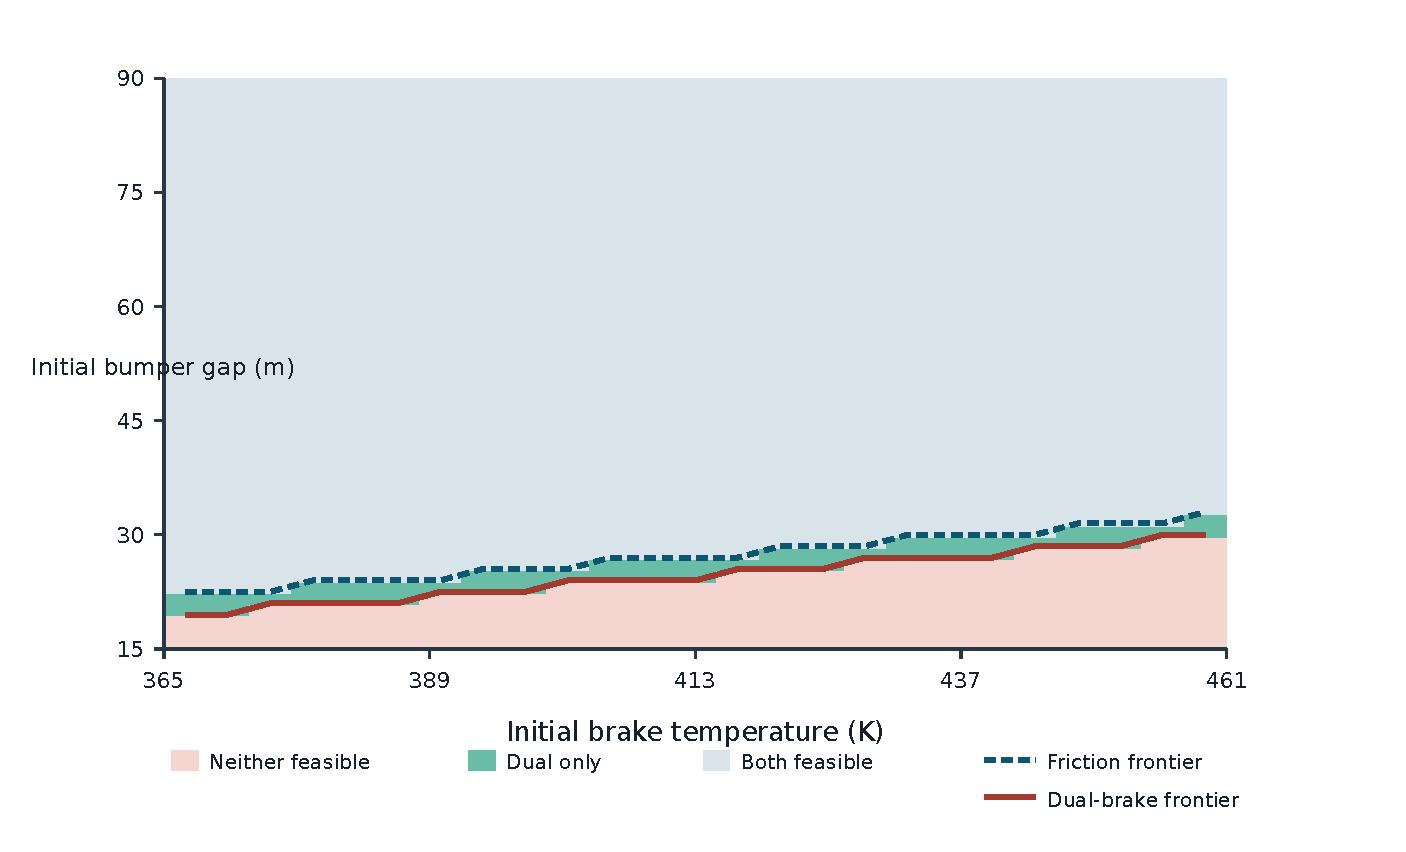
\includegraphics[width=.85\textwidth]{../generated/submission_revision/figures/feasibility_frontier.pdf}
\caption{Initial-command feasibility frontier at 15~m/s on a 10\% downgrade. Color classifies the declared two-command hard set at each initial temperature and bumper gap; dashed and solid lines mark the friction-only and dual-brake zero-reserve boundaries within the sampled domain. The green band is feasible only with auxiliary braking.}
\label{fig:feasibility-frontier}
\end{figure*}

All four M2 allocation strategies experience a negative minimum $\rho$ (Table~\ref{tab:phase2m-controller}); hence no strategy is described as universally safe. Allocation materially changes friction/auxiliary energy, tracking error, and peak temperature, but those matched model outcomes do not identify a learning advantage. M3 further records earlier certificate loss as the specified initial brake temperature approaches $T_{\rm crit}$; exact loss times and first critical components appear in Table~\ref{tab:final-model-evidence}.

A same-domain ablation retains the plant, hard rows, nominal dual-brake controller, disturbances, communication, and initial state while removing predictive/upstream triggering from the supervisor. In three 100-step, three-truck pairs, both versions have zero hard-certificate losses in ordinary and hot descents; both have six loss samples in the leader-braking case. Minimum reserves are identical within each pair (0.059, 0.023, and $-2.076$). Anticipatory mode is activated for 156, 300, and 294 truck-samples only in the proposed version, but this design does not show a closed-loop certificate-loss reduction. The full matched rows and comparison code are supplied with the source.

\begin{table*}[!t]
\centering\scriptsize
\caption{Selected model-based evidence from the Phase 2M analysis.}
\label{tab:final-model-evidence}
\begin{tabular}{llll}
\toprule
Study & Quantity & Result & Interpretation \\
\midrule
M1 & Dual/friction feasible points & 270/288; 270/288 & No feasible-count increase \\
M1 & Positive dual-reserve gain & 192/288 & Margin improvement only \\
M3 & Certificate loss at $T_0=413.7$ K & 16.4 s & collision\_demand \\
M3 & Certificate loss at $T_0=453.7$ K & 11 s & collision\_demand \\
M3 & Certificate loss at $T_0=461.7$ K & 10 s & collision\_demand \\
\bottomrule
\end{tabular}
\end{table*}

\begin{table*}[!t]
\centering
\scriptsize
\caption{Matched long-descent deterministic controller comparison.}
\label{tab:phase2m-controller}
\begin{tabular}{lrrrrr}
\hline
Method & Peak T (K) & Min. rho & Friction energy (MJ) & Auxiliary energy (MJ) & Speed root-mean-square error (m/s) \\
\hline
fixed\_auxiliary\_first & 458.81 & -28.532 & 12.265 & 25.978 & 2.8775 \\
fixed\_friction\_first & 458.8 & -10.141 & 13.233 & 24.796 & 2.3195 \\
friction\_only & 364.36 & -364.1 & 1.1293 & 0 & 15.938 \\
qp\_dual\_brake & 458.83 & -17.98 & 12.812 & 25.258 & 2.5585 \\
\hline
\end{tabular}
\end{table*}


\subsection{Predictive, Robustness, Communication, and Low-Speed Evidence}
The M4 case has neither a predictive crossing nor an observed instantaneous boundary, so it is inconclusive. M5 verifies the minimum-over-prefix horizon relation for every stored record; longer horizons can decrease the numerical predictive value, as Table~\ref{tab:phase2m-predictive} shows.

\begin{table*}[!t]
\centering
\scriptsize
\caption{Predictive-monitor and horizon metrics.}
\label{tab:phase2m-predictive}
\begin{tabular}{lrrrrrl}
\hline
Case & Trigger (s) & Boundary (s) & Warning (s) & Vehicle & Step & Component/status \\
\hline
M4 & -- & -- & -- & 1 & 3 & friction\_interval \\
M5 H=1 & -- & -- & -- & -- & -- & prefix monotonic=True \\
M5 H=3 & -- & -- & -- & -- & -- & prefix monotonic=True \\
M5 H=5 & 0 & -- & -- & -- & -- & prefix monotonic=True \\
M5 H=10 & 0 & -- & -- & -- & -- & prefix monotonic=True \\
\hline
\end{tabular}
\end{table*}


The targeted follow-up contains \FollowupScenarioCount{} boundary-approach scenarios: \FollowupTrueWarningCount{} isolated early warnings, \FollowupConservativeWarningCount{} warnings without a unique later boundary, and \FollowupSimultaneousWarningCount{} simultaneous crossings. Only \FollowupRobustTrueWarningCount{} early warnings satisfy the strict adjacent-grid and finite-margin rule. Figure~\ref{fig:predictive-examples} contrasts an isolated warning with a nonisolated case. Across 32,849 stored numerically positive predictive vehicle-samples, contemporaneous $\rho_i$ was never negative (minimum 0); this checks implementation consistency but not the sound-enclosure premise of Proposition~2. The tube regression checks 5,000 sampled states, not all future reachable states. A negative predictive value is an inconclusive warning, not proof of future infeasibility.

\begin{figure*}[t]
\centering
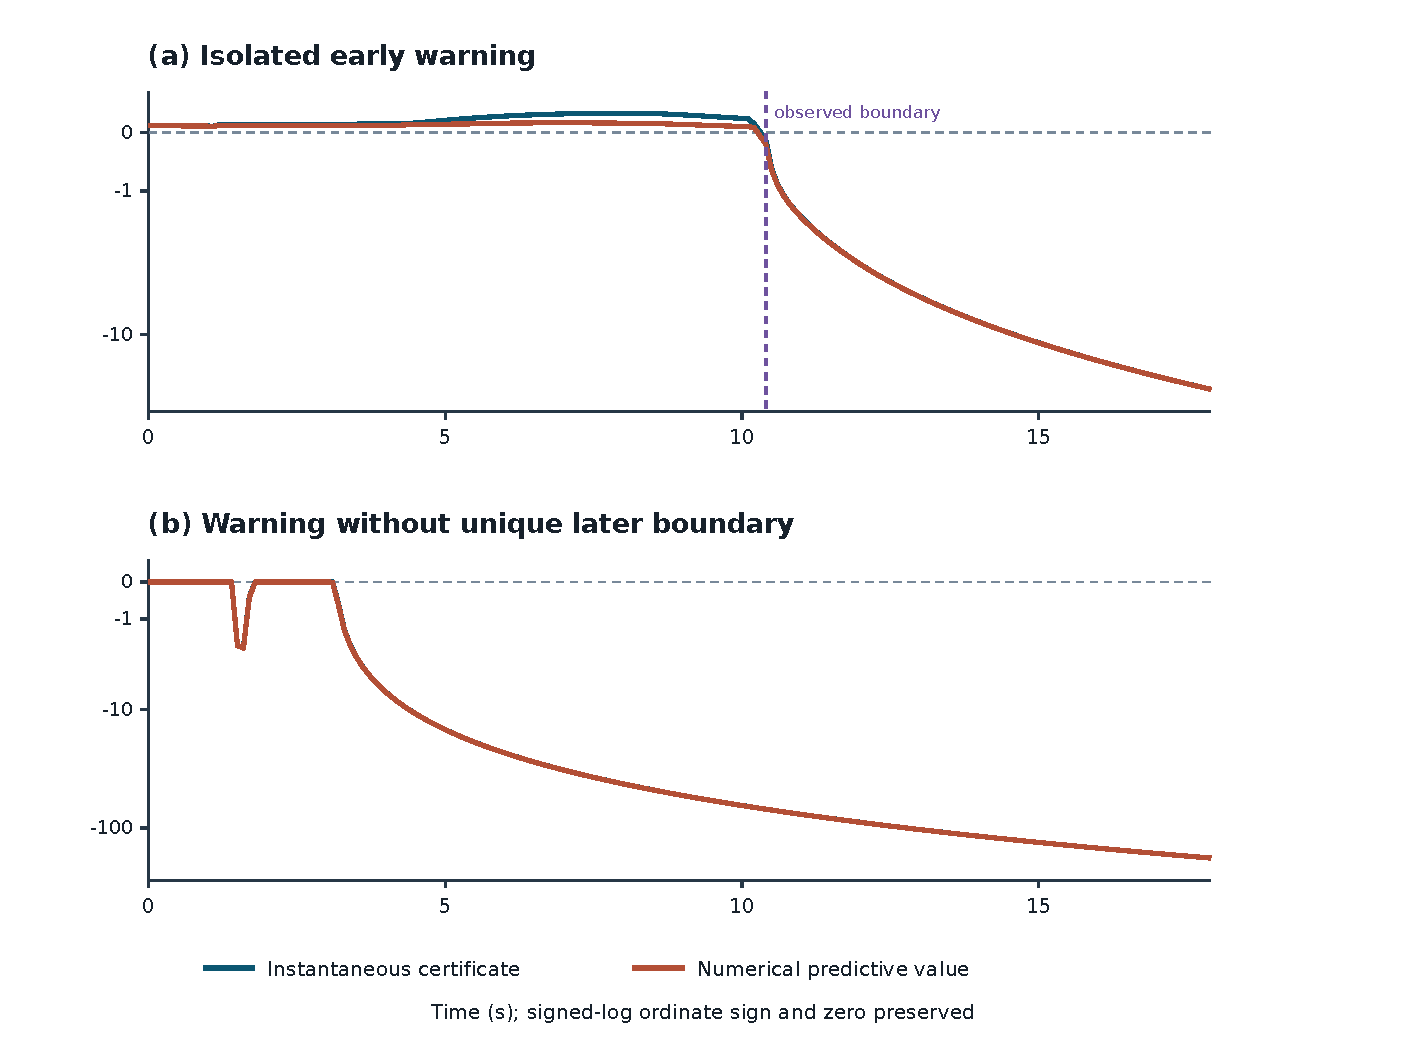
\includegraphics[width=.8\textwidth]{../generated/submission_revision/figures/predictive_examples.pdf}
\caption{Follower-1 instantaneous reserve and numerical predictive value in one isolated early-warning case (top) and one warning without a unique later boundary (bottom). The signed-log vertical mapping preserves the zero crossing while displaying the large negative tails; curves are model-based traces, not verified robust reachable-set bounds.}
\label{fig:predictive-examples}
\end{figure*}

M6 does not support a universal robustness claim. The deterministic endpoint set includes a certificate loss, and three of the 20 joint design-sensitivity samples lose the certificate. The joint set is not a physical probability distribution, so its loss frequency is not a reliability estimate; complete rows remain in the reproducibility package.

A separate 300-point stratified design varies the provenance-bounded mass, friction lag, cooling, and friction-force limit, plus auxiliary-capacity scale and digitization-bound fade-temperature offset around the 413-K/24-m boundary state. It yields 133 nonnegative initial reserves, with minimum $-1.505$ and maximum 0.059; collision demand limits 172 points and the auxiliary interval 128. This exposes sensitivity of boundary membership and normalized attribution, rather than a failure probability. Thermal capacity and auxiliary lag are held fixed because their declared intervals have zero width.

M7 and new fixed-delay runs quantify the cost of stale fleet awareness. At the head truck, mean absolute deviation from the centralized oracle grows from $3.1\times10^{-6}$ at zero delay to 0.027, 0.055, and 0.078 at 100, 200, and 300~ms. Under the 100-ms sample/consume schedule, nominal 50 and 100~ms configurations yield the same effective age and measured outcome. Head-truck critical-vehicle agreement drops from 1.00 at zero delay to 0.62, 0.64, and 0.62, respectively. The corresponding head missed/false trigger counts are 9/8, 7/10, and 6/11; therefore these counts are not monotone with delay, even though mean reserve error rises. Bounded-delay and stale-message cases reach a 1.118 mean head gap and 112 false triggers each. Figure~\ref{fig:communication} shows the deviation; the full channel metrics are archived. Vehicle-level agreement over all followers is lower even at zero delay because a non-head truck only aggregates its own upstream subchain.

\begin{figure*}[t]
\centering
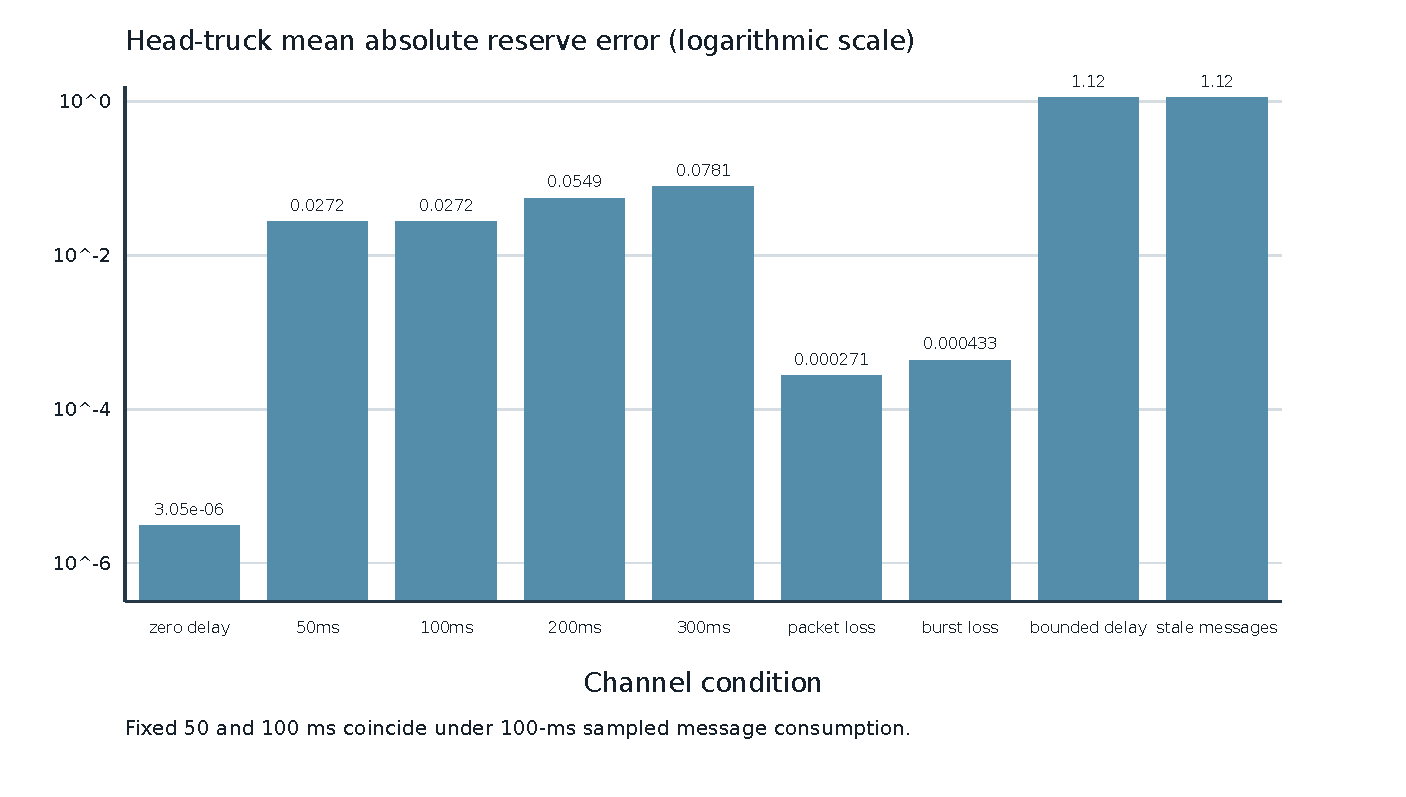
\includegraphics[width=.8\textwidth]{../generated/submission_revision/figures/communication_age.pdf}
\caption{Head-truck mean absolute deviation between the age-aware recursive reserve and instantaneous centralized oracle across fixed-delay and loss/staleness cases (logarithmic vertical scale). Each case contains 120 head-truck samples; the 50- and 100-ms delay cases coincide under 100-ms sampled consumption.}
\label{fig:communication}
\end{figure*}

M8 finds finite row evaluations but a hot-brake reserve jump across $v_\epsilon$: the ZOH and high-order barrier branches are different sufficient conditions, and their normalized reserves need not match. Because a smooth interpolation of sufficient conditions would not preserve the exact feasibility statement, we retain the hard switch and do not infer a physical feasibility discontinuity from its magnitude. The supervisor uses the actually active branch and reverifies every changed command. M9 does not satisfy the pre-registered numerical string-stability criterion in the tested grade-transition cases; string stability is an orthogonal performance property, not a theorem established here.

M10 measures computation only on the recorded Windows/Python test platform. The worst tested 99th-percentile controller time (P99) is below the 100-ms sampling period; component-wise measurements remain in the source package. This is neither target-hardware certification nor a real-time guarantee.

\subsection{Formal Learning and Conditional Differentiation}
Regular-case tests validate the local KKT derivative, but the calibrated paired-learning regime activates nonregular QP sets on every tested sample: the gradient-valid fraction is \FinalGradientValid{} and the fallback fraction \FinalFallback{}. DiffQP and matched StopGradient consequently have identical recorded returns and intervention outcomes in this campaign, with no evidence of a learning advantage. The forward safety projection remains unchanged. Detailed ten-seed protocol, paired outcomes, and gradient diagnostics are provided in the reproducibility package rather than promoted as a main feasibility result.

\subsection{Adapted External-Baseline Comparison}
The six deterministic matched heavy-duty transfer pairs have zero geometric collisions under both methods. The proposed method has lower peak brake temperature in each pair (362.43--461.71~K versus 479.24--658.92~K for the adapted Zhou \emph{et al.} controller) and no fade-envelope violation, while the transferred controller records 1,139 violations in total. These observations isolate a physical constraint class omitted by the scalar-acceleration source policy under the fixed adapter; they do not rank the native algorithms. Full per-case results and adapter code accompany the source package.

The post-hoc numerical evaluation of $\rho^{H,\mathrm{cert}}$ is negative for the adapted baseline in all six cases. The proposed method has negative predictive-monitor values in four cases and nonnegative values in two, so neither unconditional feasibility nor universal predictive superiority follows. Rather, the common feasibility monitor exposes collision--thermal conflicts that are not represented explicitly by the transferred collision-centric controller.

Lower speed root-mean-square error (RMSE), spacing RMSE, and jerk RMS are observed for the proposed method in all six matched pairs. Its traces use more auxiliary-braking energy in five cases and less friction-braking energy in all six, showing a systematic shift from friction toward auxiliary braking under the proposed allocator. These are observed deterministic matched outcomes, not general learning or energy-efficiency claims. The transferred baseline is computationally cheaper on the reported platform: its P99 runtime is 0.232--0.328~ms versus 1.037--1.522~ms. The proposed stack additionally evaluates thermal/fade hard rows, instantaneous feasibility, a predictive interval tube, a distributed bottleneck, and supervisor/reverification logic; the measured disadvantage is nevertheless retained and is not target-hardware real-time certification.

This comparison is adapter-sensitive because the source method outputs scalar acceleration while the heavy-duty plant requires friction/auxiliary commands. Observation mapping, the absence of heavy-duty retraining, and independently prespecified choices for unreported source details also affect the transfer. It is therefore a matched domain-transfer stress test, not a complete ranking of the algorithms in their native domains.

\section{Discussion and Limitations}
The primary contribution is feasibility certification and physical conflict attribution. The geometry makes the source of a feasibility loss inspectable: raising temperature contracts the friction interval; auxiliary braking may restore command authority, but only up to its own gear, speed, power, and lag bounds. The targeted frontier demonstrates a nonempty dual-only band under specified initial conditions, whereas the matched closed-loop ablation shows that predictive triggering need not reduce certificate losses in every tested disturbance. A certificate can therefore distinguish \emph{available authority} from \emph{realized supervisory benefit}. Its sign is invariant to positive normalizer changes, but limiting-component attribution is normalized: across the 288 M1 states, varying one of $s_f,s_a,s_M$ by 0.5 or 2 preserves every sign while component agreement ranges from 0.896 to 1.000. Trigger-time sensitivity was not measured and is not inferred from those snapshots.

Communication freshness controls the fidelity of fleet-level awareness. The head's zero-delay recursive minimum agrees with the centralized oracle, while delay, loss, and stale replacement alter both the value and its attribution. The framework can filter commands from different nominal controllers. Its theoretical finite-horizon guarantee requires sound uncertainty and reserve enclosures and final-action reverification; the present floating-point predictor lacks a verified enclosure proof. The low-speed switch remains discontinuous as a numerical certificate because its two sufficient conditions differ; no unsafe interpolation was introduced.

The plant is a literature-calibrated composite rather than an identified truck, and the lumped thermal model omits wheel-end imbalance and spatial gradients. There is no field or hardware-in-the-loop validation, analytical string-stability result, or universal closed-loop feasibility claim. Learning differentiation is secondary: persistent active-set degeneracy disables its QP-mediated backward path in the formal campaign. The external comparison is adapter-sensitive, and computation times apply only to the measured platform. These boundaries motivate identified thermal models and communication-aware validation in future work.

\section{Conclusion}
Collision avoidance, brake heating/fade, and constrained auxiliary actuation create an opposed command geometry in heavy-duty platoons. For the declared two-dimensional hard set, the instantaneous certificate is an exact nonemptiness test. Under sound enclosure assumptions, interval propagation supplies a one-sided finite-horizon extension, while the present numerical predictor lacks formal implementation assurance. An age-aware recursive minimum communicates the limiting vehicle and physical component for dual-brake supervision. A targeted initial-state frontier contains 43 dual-only feasible points among 1,275 evaluated states; matched same-plant runs isolate supervisory triggering without demonstrating a certificate-loss reduction in the three tested cases. Communication-age results quantify how delayed messages degrade fleet-feasibility awareness. The contribution is a physical feasibility and control interface independent of the nominal controller. Verified interval implementation, identified vehicle data, and field validation are the next tests of its operational reach.

\appendices
\section{Expanded Affine Rows and Checks}
For linear $\alpha_{1c}(s)=k_{1c}s$ and $\alpha_{2c}(s)=k_{2c}s$, substitution of \eqref{eq:jerk} into \eqref{eq:hcddot} gives the collision row coefficients in \eqref{eq:collision_hocbf} and the nominal uncontrolled term
\begin{align}
\widehat\Xi_i^c={}&a_{i-1}-a_i-\frac{a_i^2}{a_i^S}
-c_i\!\left(\frac{\widehat{\dot F_i^r}}{m_i}+\frac{b_i}{m_i\tau_i^f}+\frac{r_i}{m_i\tau_i^a}\right)\nonumber\\
&+\frac{a_{i-1}^2}{a_{i-1}^E}+r_{i-1}^v\widehat{\dot a}_{i-1}
+(k_{1c}+k_{2c})\dot h_i^c+k_{1c}k_{2c}h_i^c.
\end{align}
Thus the signs of both command coefficients are positive. The thermal expansion follows directly from
\begin{equation}
\ddot h_i^T=-\frac{\eta_i}{C_i}(\dot b_iv_i+b_ia_i)
+\frac{k_i}{C_i}(\dot T_i-\dot T_a)-\frac{\dot q_i^w}{C_i},
\end{equation}
and $\dot b_i=(-b_i+u_i^f)/\tau_i^f$, which gives the negative friction-command coefficient in \eqref{eq:thermal_hocbf}. For fade,
\begin{equation}
\dot h_i^F=\bar b_i\phi_i'(T_i)\dot T_i+\frac{b_i-u_i^f}{\tau_i^f},
\end{equation}
whose rearrangement is exactly \eqref{eq:fade_cbf}.

For the auxiliary envelope, $\dot h_i^A=\bar r_{i,v}a_i+(r_i-u_i^a)/\tau_i^a$; rearranging $\dot h_i^A+\alpha_A(h_i^A)\ge\gamma_i^A+\mu_i^A$ gives \eqref{eq:auxcbf}. For the low-speed row, variation of constants applied to the cascaded first-order friction actuator and thermal state produces the kernels $I_{0i}$ and $I_{1i}$ in \eqref{eq:zohthermal}. Since $I_{0i}-I_{1i}\ge0$, the row is an upper bound on $u_i^f$ for $v_i>0$ and degenerates continuously to $0\le g_{i,k}^{T0}$ at $v_i=0$. The latter term is retained independently in \eqref{eq:rho}, so a negative state-only reserve cannot be hidden by nonempty command intervals.

Jerk follows from \eqref{eq:jerk} and is logged as a comfort outcome, but it contributes no row, slack, or decision variable to \eqref{eq:qp}. The symbolic suite independently verifies collision and thermal differentiation, command coefficients, and fade/auxiliary rearrangements. The randomized equation-regression script draws 10,000 physical cases for each of five families: collision differentiation/affine/QP agreement, thermal differentiation/affine/QP agreement, fade rearrangement, auxiliary-envelope rearrangement, and exact-reserve agreement. It also checks zero/near-zero-speed ZOH boundaries. A dedicated low-speed suite covers $v=0$, $v\approx0$, $v=v_\epsilon$, and $v>v_\epsilon$ under hot and cold initial brakes; verifies mutually exclusive HOCBF/ZOH partitioning; and confirms that $g^{T0}<0$ alone makes both the hard row and complete certificate infeasible when the command coefficient is zero. A separate predictive suite compares the complete instantaneous conjunction against 10,000 independent interval-box LP vertex solves; verifies $H=1$ reduction under zero uncertainty; checks 5,000 Monte Carlo sampled states against the interval tube; and checks fleet min/argmin and anticipatory triggering. These tests detect implementation regressions but do not identify uncertainty bounds, prove continuous-time containment, establish arbitrary state-feedback monotonicity, or replace vehicle validation.


\bibliographystyle{IEEEtran}
\bibliography{references}
\end{document}
